%-----------------------------------------------
% Dateiname: Thesis.tex
% Autor    : Stefano Kowalke <blueduck@gmx.net>
% Lizenz   : BSD
%-----------------------------------------------

%-------------------------
% Importiere die Präambel
%-------------------------
%-----------------------------------------------
% Dateiname: Thesis-Preamble.tex
% Autor    : Stefano Kowalke <blueduck@gmx.net>
% Lizenz   : BSD
%-----------------------------------------------

%----------------------------------
% Dokumentenklasse DINA4 einseitig
%----------------------------------
\documentclass[
	fontsize    = 11pt,           % Die Schriftgröße
	twoside     = false,          % scrbook hat per Default ein Zwei-Seitenlayout
	parskip     = full,           % Steuert die Absätze. http://www.rrzn.uni-hannover.de/fileadmin/kurse/material/latex/scrguide.pdf Tabelle 3.7
	headsepline,                  % Fügt eine Trennungslinie in den Seitenkopf
	footnotes   = multiple,       % Fügt ein Komma zwischen den Indexzahlen bei aufeinanderfolgende Fußnoten ein
	numbers     = noendperiod     % Keinen Punkt der letzten Gliederungsebene in der Überschrift  -> 1.2.1 statt 1.2.1.
]{scrbook}

%\includeonly{Chapters/Doctrine}
\PassOptionsToPackage{
    %layout,
    drafting,
    eulerchapternumbers,
    eulermath,
    colophon,
    bettertable,
    %minionpro,
    %dottedtoc,
}{thesis}


%===============
% Pakete laden
%===============
\usepackage{fontspec}                      % Wird von LuLaTeX benöigt und löst "fontenc" ab.
\usepackage{polyglossia}                   % Wird von LuLaTeX benöigt und löst "babel" ab.
\usepackage[german=quotes]{csquotes}       % Anführungszeichen global im Dokument steuern. Paket wird von "polyglossia" empfohlen.

\usepackage[
	backend=biber,                         % Benutzer biber zur Erstellung
	bibwarn=true,                          % Warne, wenn das BiTex Format falsch ist
	autolang=other,
	style=alphabetic-verb,
	bibstyle=alphabetic-verb,
]
{biblatex}                                 % Nutze Biblatex zur Erstellung des Literaturverzeichnis
\addbibresource{Bib/Bibliography.bib}      % Die Literatureinträge
\usepackage{minted}                        % Sourcecode Highlighting. Dieses Package benötigt Python und Pygments 1.5. Version 1.6 macht Probleme mit gerade Anführungszeichen (') - es stellt sie als normale Anführungszeichen dar.
\usepackage[punct-after=true]{fnpct}       % Ermöglicht das Setzen der Indexzahlen der Fußnoten hinter dem Punkt oder Komma. Hier ist es dafür gedacht die Option footnotes=multiple von KOMA wiederherzustellen, die durch das Hyperref Paket kaputt gegangen ist.
\usepackage{hyperref}                      % Stellt Links in Schreibmaschinenschrift dar und legt einen Link über den Text.
                                           % Dieses Package sollte als letztes aufgerufen werden, da es Problem mit Anderen geben könnte
\usepackage[
    xindy={language=german,codepage=din5007-utf8}, % Ruft Xindy zum Erstellen des Index in der deutschen Version auf
    toc,                                   % Fügt die Glossare dem Inhaltsverzeichnis zu
    acronym,                               % Erstellt ein neues Glossar mit dem Label "acronym"
    nonumberlist,                          % Fügt die Seitenzahlen hinzu, auf denen der Eintrag vorkommt, nicht hinzu
    nopostdot                              % Entferne den Punkt am Ende der Definition
    ]{glossaries}                          % Erstellt Glossar und Abkürzungsverzeichnis. Laut der Dokumentation ist es ausdrücklich notwendig, dass es nach dem Package hyperref eingebunden werden muß
\makeglossaries                            % Anweisung das Glossar zu erstellen

\newfontfamily\quotefont[Ligatures=TeX]{Palatino} % The font for the quotation marks at a quote

\usepackage{chronosys} % Creates timelines

%=================================================
% Angaben zur Arbeit wie Titel und Name des Autor
%=================================================
\newcommand{\myTitle}{Integration der Datenbank-Abstraktionsschicht Doctrine2\xspace}
\newcommand{\myTitleSecondLine}{in das Content-Management-System TYPO3\xspace}
%\newcommand{\mySubtitle}{Put your subtitle here\xspace}
%\newcommand{\myDegree}{Put your degree here\xspace}
\newcommand{\myName}{Stefan Kowalke\xspace}
\newcommand{\myEMail}{<stefan.kowalke@stud.fh-flensburg.de>\xspace}
\newcommand{\myMatricleNumber}{485366\xspace}
\newcommand{\myProf}{Prof. Dr. Hans-Werner Lang\xspace}
\newcommand{\myOtherProf}{Dipl. VK Tobias Hiep\xspace}
%\newcommand{\mySupervisor}{Put name here\xspace}
\newcommand{\myUni}{\uppercase{\large Fachhochschule Flensburg}\xspace}
\newcommand{\myDepartment}{Angewandte Informatik\xspace}
%\newcommand{\myFaculty}{Put data here\xspace}
\newcommand{\myMajor}{Medieninformatik\xspace}
\newcommand{\myLocation}{Flensburg\xspace}
\newcommand{\myTime}{März 2014\xspace}
%\newcommand{\myVersion}{version 4.1\xspace}


%----------------
% Renew commands
%----------------
%\renewcommand*{\multfootsep}{,\nobreakspace}  % Fügt bei den hochgestellten Indexzahlen von Fußnoten ein Leerzeichen nach dem Komma ein
\deffootnote{1em}{1em}{\thefootnotemark\ }    % Setzt die Indexzahlen in den Fußnoten etwas entfernt vom Text

%---------------------------------------------------------------
% Renew the citation style from parenthesis to square brackets:
%---------------------------------------------------------------
% (Popel 2007, S. 59–63) -> [Popel 2007, S. 59–63]
% http://tex.stackexchange.com/questions/16765/biblatex-author-year-square-brackets
%---------------------------------------------------------------
\makeatletter
\newrobustcmd*{\parentexttrack}[1]{%
  \begingroup
  \blx@blxinit
  \blx@setsfcodes
  \blx@bibopenparen#1\blx@bibcloseparen
  \endgroup}

\AtEveryCite{%
  \let\parentext=\parentexttrack%
  \let\bibopenparen=\bibopenbracket%
  \let\bibcloseparen=\bibclosebracket}
\makeatother

%----------------------
% Neue Quoting Umgebung
%----------------------
\newcommand*\quotesize{60} % if quote size changes, need a way to make shifts relative
% Make commands for the quotes
\newcommand*{\openquote}
   {\tikz[remember picture,overlay,xshift=-4ex,yshift=-2.5ex]
   \node (OQ) {\quotefont\fontsize{\quotesize}{\quotesize}\selectfont``};\kern0pt}

\newcommand*{\closequote}[1]
  {\tikz[remember picture,overlay,xshift=4ex,yshift={#1}]
   \node (CQ) {\quotefont\fontsize{\quotesize}{\quotesize}\selectfont''};}

% select a colour for the shading
\definecolor{shadecolor}{gray}{0.95}

\newcommand*\shadedauthorformat{\emph} % define format for the author argument

% Now a command to allow left, right and centre alignment of the author
\newcommand*\authoralign[1]{%
  \if#1l
    \def\authorfill{}\def\quotefill{\hfill}
  \else
    \if#1r
      \def\authorfill{\hfill}\def\quotefill{}
    \else
      \if#1c
        \gdef\authorfill{\hfill}\def\quotefill{\hfill}
      \else\typeout{Invalid option}
      \fi
    \fi
  \fi}

% wrap everything in its own environment which takes one argument (autor) and one 
% optional argument [l, c or r]
\newenvironment{shadequote}[2][l]%
{\authoralign{#1}
\ifblank{#2}
   {\def\shadequoteauthor{}\def\yshift{-2ex}\def\quotefill{\hfill}}
   {\def\shadequoteauthor{\par\authorfill\shadedauthorformat{#2}}\def\yshift{2ex}}
\begin{snugshade}\begin{quote}\openquote}
{\shadequoteauthor\quotefill\interlinepenalty=10000\end{quote}\end{snugshade}}

%------------------
% Eigene Kommandos
%------------------


%---------------------
% Spracheinstellungen
%---------------------
\setdefaultlanguage[spelling=new]{german}   % Die Sprache muß vor dem Einbinden von dem Blindtextpackage eingestellt werden
\usepackage{blindtext}                      % Erstellt schnell und einfach Blindtexte mit \Blindtext. Wird ausnahmsweise hier eingebunden


%-------------------
% Linkkonfiguration
%-------------------
\hypersetup
{
	pdftitle       = {\myTitle \myTitleSecondLine},
	pdfauthor      = {\myName},
	pdfsubject     = {\myTitle \myTitleSecondLine},
	pdfcreator     = {\myName},
	pdfkeywords    = {typo3} {dbal} {doctrine} {mysql} {postgres},
	linktoc        = all,
	colorlinks     = true,
	linkcolor      = black,
	citecolor      = black,
	filecolor      = black,
	urlcolor       = blue,
}

%----------
% Grafiken
%----------
\graphicspath{ {gfx/} }

%--------------
% Code Listing
%--------------
%**************************************
% Schrifteinstellungen für Codelistings
\setmonofont[Scale=0.75]{Source Code Pro}
\definecolor{bg}{rgb}{0.95,0.95,0.95}
\newminted{php}{
	linenos              = true,
	xleftmargin          = 2em,
	tabsize              = 4,
	bgcolor              = bg,
	funcnamehighlighting = true
}

\newminted{mysql}{
	linenos     = true,
	bgcolor     = bg,
	xleftmargin = 2em
}

\usepackage{thesis}


%--------------------------------
% Importiere die Glossareinträge
%--------------------------------
%-----------------------------------------------
% Dateiname: Definitions.tex
% Autor    : Stefano Kowalke <blueduck@gmx.net>
% Lizenz   : BSD
%-----------------------------------------------

%-----------------
% Abkürzungen
%-----------------
% http://tex.stackexchange.com/questions/8946/how-to-combine-acronym-and-glossary

\newglossaryentry{t3assoc}
{
	type=\acronymtype,
	name={T3Assoc},
	description={TYPO3 Association},
	first={TYPO3 Association (T3Assoc)},
}

\newglossaryentry{dbal}
{
	type=\acronymtype,
	name={DBAL},
	description={Database Abstraction Layer},
	first={Database Abstraction Layer (DBAL)},
	see=[Glossary:]{dbalg}
}

\newglossaryentry{bafög}
{
	type=\acronymtype,
	name={BAföG},
	description={Bundesausbildungsförderungsgesetz},
	first={Bundesausbildungsförderungsgesetz (BAföG)}
}

\newglossaryentry{cms}
{
	type=\acronymtype,
	name={CMS},
	description={Content-Management-System},
	first={Content-Management-Sytem (CMS)}
}
\newglossaryentry{ecms}
{
	type=\acronymtype,
	name={ECMS},
	description={Enterprise Content Management-System},
	first={Enterprise Content Management-Sytem (ECMS)}
}

\newglossaryentry{wcms}
{
	type=\acronymtype,
	name={WCMS},
	description={Web Content Management-System},
	first={Web Content Management-Sytem (WCMS)}
}

\newglossaryentry{orm}
{
	type=\acronymtype,
	name={ORM},
	description={Object-relational mapping},
	first={Object-relational mapping (ORM)}
}

\newglossaryentry{jcr}
{
	type=\acronymtype,
	name={JCR},
	description={Content Repository for Java Technology API},
	first={Content Repository for Java Technology API (JCR)}
}

\newglossaryentry{mvc}
{
	type=\acronymtype,
	name={MVC},
	description={Model-View-Controller},
	first={Model-View-Controller (MVC)}
}

\newglossaryentry{api}
{
	type=\acronymtype,
	name={API},
	description={Application Programming Interface},
	first={Application Programming Interface (API)}
}

\newglossaryentry{apis}
{
	type=\acronymtype,
	name={APIs},
	description={Application Programming Interface},
	first={Application Programming Interface (API)}
}

\newglossaryentry{gpl2}
{
	type=\acronymtype,
	name={GPL2},
	description={GNU General Public License v.2},
	first={GNU General Public License v.2 (GPL2)}
}

\newglossaryentry{cmf}
{
	type=\acronymtype,
	name={CMF},
	description={Content Management Framework},
	first={Content Management Framework (CMF)}
}
%-------------
% glossareinträge
%-------------
\newglossaryentry{dbalg}
{
	name={dbal},
	description={a very long description of of what is dbal}
}


%--------------------------------------
% Hier fängt der eigentliche Inhalt an
%--------------------------------------
\begin{document}
	\frontmatter
		%-----------------------------------------------
% Dateiname: Titlepage.tex
% Autor    : Stefano Kowalke <blueduck@gmx.net>
% Lizenz   : BSD
%-----------------------------------------------
\begin{titlepage}
	\begin{center}
		\myUni\\
	\end{center}
	\begin{center}
		\large Fachbereich \myDepartment
	\end{center}
	\begin{verbatim}


	\end{verbatim}
	\begin{center}
		\uppercase{\textbf{\large Bachelorthesis}}
	\end{center}
	\begin{verbatim}
	\end{verbatim}
	\begin{center}
		\textbf{im Studiengang \myMajor}
	\end{center}
	\begin{verbatim}







	\end{verbatim}
	\begin{flushleft}
		\begin{tabular}{lll}
			\textbf{Thema:} & & \myTitle \\
			&&  \myTitleSecondLine \\
			& & \\
			& & \\
			& & \\
			\textbf{eingereicht von:} & & \myName\ \myEMail\\
			& & \\
			& & \\
			\textbf{Matrikelnummer:} & & \myMatricleNumber\\
			& & \\
			& & \\
			\textbf{Abgabedatum:} & & \today\\
			& & \\
			& & \\
			\textbf{Erstprüfer:} & & \myProf\\
			& & \\
			& & \\
			\textbf{Zweitprüfer:} & & \myOtherProf
		\end{tabular}
	\end{flushleft}
\end{titlepage}

		%-----------------------------------------------
% Dateiname: Colophon.tex
% Autor    : Stefano Kowalke <blueduck@gmx.net>
% Lizenz   : BSD
%-----------------------------------------------
\thispagestyle{empty}
\vspace*{\fill}
\begin{flushleft}
    \sffamily
    \footnotesize
    \noindent
Dieses Dokument wurde am \today\ mit \InfoLaTeX\ gesetzt.
    \par\bigskip\noindent
    \begin{tabular}{ll}
Schrift: & {Palatino 10pt}\\
Typographie: & \KOMAScriptVersion\\
System: & \InfoTeX\ auf OSX 10.8\\
Editor: & Mou 0.8.5 beta und VIM 7.4 \\
    \end{tabular}
    \par\bigskip\noindent
    {Es steht unter der \textbf{Creative Commons Namensnennung – Weitergabe unter gleichen Bedingungen 4.0 International Lizenz}} und kann unter \url{https://github.com/Konafets/thesis} heruntergeladen werden.
    \begin{figure}[h!]
        \centering
        \includegraphics[scale=0.75]{by-sa.eps}
     \end{figure}\\
     Der für diese Thesis entstandene Prototyp steht unter der \textbf{GNU General Public License version 2 oder neuer} \url{http://www.gnu.org/licenses/gpl-2.0.html} und ist unter \url{https://github.com/Konafets/ext-doctrine_dbal} zu finden.

     TYPO3 CMS steht unter der \textbf{GNU General Public License version 2 oder neuer} \url{http://www.gnu.org/licenses/gpl-2.0.html}. Die modifizierte Version ist unter \url{https://github.com/Konafets/TYPO3CMSDoctrineDBAL} zu finden.
     \\[1\baselineskip]

	 Das Latex-Template basiert auf der ClassicThesis von André Miede zu finden unter \url{http://www.miede.de/index.php?page=classicthesis}. Es steht unter der \textbf{GNU General Public License} \url{http://www.gnu.org/copyleft/gpl.html}.
     \\[1\baselineskip]

	 \textit{The Joy of Programming with Bob Ross} von Abstruse Goose zu finden unter \url{http://abstrusegoose.com/467} steht unter der Lizenz \textbf{Attribution-NonCommercial 3.0 United States (CC BY-NC 3.0 US)} \url{http://creativecommons.org/licenses/by-nc/3.0/us/}.
     \\[1\baselineskip]
	 \textit{Exploits of a mom} von xkcd zu finden unter \url{http://xkcd.com/327/} steht unter der Lizenz \textbf{Attribution-NonCommercial 2.5 Generic (CC BY-NC 2.5)} \url{http://creativecommons.org/licenses/by-nc/2.5/}.
\end{flushleft}
\normalsize

		%-----------------------------------------------
% Dateiname: Abstract.tex
% Autor    : Stefano Kowalke <blueduck@gmx.net>
% Lizenz   : BSD
%-----------------------------------------------
\chapter{Abstract}
\label{ch:abstract}
Webanwendungen werden häufig um ein Datenbankmanagementsystem herum entworfen. In der Vergangenheit war dies oft MySQL. Um eine Webanwendung aus der Abhängigkeit zu einem spezifischen Datenbankmanagementsystem zu lösen, kann die, von PHP mitgelieferte, Datenbankabstraktionsschicht PDO genutzt werden. Einen Schritt weiter geht Doctrine DBAL, welches – auf PDO aufbauend – eine einheitliche Schnittstelle zu weiteren Datenbankmanagementsystemen bereitstellt. Doctrine DBAL ist zudem die Grundlage für Doctrine ORM - ein Framework zur Objekt-relationalen Abbildung von Objekten auf eine Datenbank, das in TYPO3 Flow und TYPO3 Neos eingesetzt wird. Diese Arbeit demonstiert wie durch die Integration von Doctrine DBAL in das Content-Manangement-System TYPO3 CMS die Abhängigkeit zu MySQL entfernt werden kann.

		\newpage
		\thispagestyle{empty}
		\hspace{1cm}
		\newpage
		\thispagestyle{empty}
		\vspace*{\fill}
		\begin{verse}
			\centering
			``'The Babel fish,' said The Hitchhiker's Guide to the Galaxy quietly, 'is small, yellow and leech-like, and probably the oddest thing in the Universe.\\
			...\\
			The practical upshot of all this is that if you stick a Babel fish in your ear you can instantly understand anything in any form of language.'''

			– Douglas Adams, The Hitchhiker's Guide to the Galaxy
			%``War is peace.\\
			%Freedom is slavery.\\
			%Ignorance is strength.''

			%– George Orwell, 1984
		\end{verse}
		%\begin{quote}
			%\hfill ``@WilliamShatner Yes, Standard Orbit, Captain. And we're detecting signs of life on the surface.''\\
			%\\
			%\hfill – William Shatner und ISS Commander Chris Hadfield am 03.01.2013 auf Twitter (\url{https://twitter.com/Cmdr_Hadfield/status/286948264236945408})
		%\end{quote}
		%\begin{quote}
			%\hfill ``'The Answer to the Great Question\ldots~Of Life, the Universe and Everything\ldots~Is\ldots~Forty-two,' said Deep Thought, with infinite majesty and calm.''\\
			%\\
			%\hfill – Douglas Adams, The Hitchhiker's Guide to the Galaxy

		%\end{quote}
		\vspace*{\fill}
		\newpage
		\tableofcontents
	\mainmatter
		%-----------------------------------------------
% Dateiname: Introduction.tex
% Autor    : Stefano Kowalke <blueduck@gmx.net>
% Lizenz   : BSD
%-----------------------------------------------
\chapter{Einleitung}
\label{ch:intro}
Das Content Management System TYPO3 CMS nutzt standardmäßig die Datenbank MySQL. Wird stattdessen ein anderes Datenbank Management System wie Postgres, Oracle oder MSSQL verwendet, muss die optionale TYPO3 CMS Systemextension \textit{DBAL} installiert werden. Diese verwendet zur Konvertierung der SQL-Abfragen in die jeweiligen \gls{glos:sqlDialect}e die externe Bibliothek \textit{ADOdb} als Datenbankabstraktionsschicht.

Während DBAL stets an neue Versionen von TYPO3 CMS angepasst wurde, schien die Entwicklung von ADOdb im Jahr 2012 in einen Dornröschenschlaf verfallen zu sein\footnote{Erst während der Arbeit an dieser Thesis konnte wieder Aktivität bei der Entwicklung von ADOdb verzeichnet werden. \url{http://adodb.sourceforge.net/docs-adodb.htm\#changelog}}, was innerhalb der TYPO3 Entwicklergemeinschaft die Frage nach einem Nachfolger der Abstraktionsschicht aufwarf. Als Kanditaten kamen die Projekte PDO\footnote{\url{http://www.php.net/manual/de/book.pdo.php}}, Propel\footnote{\url{http://propelorm.org/}} und Doctrine\footnote{\url{http://doctrine-project.org}} in Frage. Am Ende konnte Doctrine überzeugen, da es unter aktiver Entwicklung steht und als einziges Projekt die Datenbankabstraktionsschicht von der Komponente der objektrealationale Abbildung voneinander getrennt anbietet. Nicht zuletzt waren die weite Verbreitung und die guten Erfahrungen, die die Schwesterprojekte von TYPO3 CMS, TYPO3 Flow und TYPO3 Neos, sammelen konnten ausschlaggebend.

Aber wie sieht es mit der Integration von Doctrine DBAL in TYPO3 CMS aus? Kann die Integration unter Beibehaltung der Kompatibilität zur existierenden Datenbank API realisiert werden? Und ist es möglich die Nutzung von Prepared Statements so weit zu vereinfachen, dass sie bevorzugt benutzt werden?

Um diese Fragen zu beantworten, soll im Rahmen der Bachelor-Thesis ein Prototyp erstellt werden, der Doctrine DBAL in TYPO3 CMS integriert und zudem eine abstrakte Abfragesprache implementiert, die eine wahlweise Benutzung von Prepared Statements ermöglicht. Als Ergebnis wird die komplette Auflösung der Abhängigkeit von TYPO3 CMS zu MySQL angestrebt. Ferner soll durch die Einführung einer abstrakten Abfragesprache die Benutzerschnittstelle mit der Datenbank vereinfacht und durch die Möglichkeit der Verwendung von Prepared Statements, die Sicherheit vor SQL-Injections erhöht werden.

Die Arbeit ist in vier Teile unterteilt:

Nach der Einführung folgt mit Kapitel zwei die Vermittlung der theoretischen Grundlagen. Es wird näher auf TYPO3 CMS, Doctrine DBAL, Prepared Statements und SQL-Injections eingegangen. Abgerundet wird das Kapitel mit der Beschreibung der Arbeitsweise und verwendeten Werkzeuge.

Im dritten Kapitel wird die Situation zu Beginn der Bachelor-Thesis beschrieben. Zur Sprache kommen die aktuelle Datenbank API, die TYPO3 CMS eigene Implementation der Prepared Statements, sowie das verwendete Datenbankschema.

Das vierte Kapitel widmet sich der Konzeption und Umsetzung des Prototypen. Es geht auf die Vorgehensweise zu dem anfänglichen Refactoring ein und beschreibt die Erstellung des Prototypen sowie dessen Integration in den Installationsprozess von TYPO3 CMS. Abgerundet wird das Kapitel mit der Implementation einer neuen Abfragesprache.

%\begin{itemize}
%\item Er ist eine normale Extension, die über das \textit{Install Tool} installierbar ist.
%\item Er ist kompatibel zur alten Datenbank API.
%\item Er ist zu 100\% kompatibel zur der Standarddatenbank MySQL.
%\item Die Namen der Methoden folgen den TYPO3 \gls{cgl}.
%\item Er führt eine abstrakte Datenabfragesprache ein, die die Benutzung von manuell formulierten SQL-Abfragen überflüssig macht.
%\item Die Abfragesprache ermöglicht die transparente Verwendung von Prepared Statements.
%\end{itemize}

%Als sich auf den Developer Days 2006 das Entwicklerteam für einen Nachfolger der eben erst erschienen TYPO3 Version 4.0 formierte (vgl.~\cite{web:berlinManifesto2008}), war wohl keinem der dort Anwesenden klar wohin die Reise gehen würde – ging man anfänglich noch von einem Refactoring\footnote{Strukturverbesserung des Quellcodes bei Beibehaltung der Funktionalität} der schon vorhandenen Codebasis aus.

%In der Konzeptionsphase kristallisierte sich immer mehr heraus, dass es damit nicht getan sein würde. Der Nachfolger mit dem Arbeitstitel ``Phoenix'' sollte nicht nur den zukünftigen Anforderungen des Web standhalten, sondern die Position der Version 4.0 weiter ausbauen. Das Entwicklerteam um Chefentwickler Robert Lemke entschloss sich die Version 5.0 des Systems komplett neu zu schreiben [Quelle anfügen] und merkte dabei, dass Entwickler bei der Programmierung von Webanwendungen immer wieder mit den gleichen Problemen wie Routing, die Erstellung und Validierung von Formularen, Login von Benutzern oder dem Aufbau einer Verbindung zur Datenbank konfrontiert werden.

%Die Idee eines – von dem Content-Management-System – unabhängigen PHP Frameworks war geboren und wurde zunächst auf den Namen FLOW3 getauft. Dieses Framework sollte die spätere Basis für TYPO3 5.0 bilden und all die oben beispielhaft angeführten wiederkehrenden Aufgaben übernehmen. Die Version 5.0 von TYPO3 sollte lediglich eins von vielen Packages darstellen mit denen FLOW3 erweitert werden kann. FLOW3 wurde daraufhin als eigenständiges ``Webapplication Framework'' konzipiert und umgesetzt, so dass es auch ohne ein \gls{cms} betrieben werden kann.

%Schon in einer recht frühen Entwicklungsphase hat man sich dem Thema Persistenz gewidmet, die zunächst noch als ``\gls{jcr}'' in PHP implementiert, jedoch später wegen zu vieler Probleme bei der Portierung der Java Spezifikation JSR-170 nach PHP durch eine eigene Persistenzschicht ersetzt wurde (vgl.~\cite{web:dambekalnsFroscamp2010}). Im weiteren Verlauf der Entwicklung kam man von dieser Idee wieder ab, da die eigene Persistenzschicht nicht performant genug war und andere Projekte wie Doctrine oder Propel schon fertige Lösungen anboten (vgl.~\cite{twitter:DoctrineFlow2014}). Schlußendlich entschied man sich für die Integration von Doctrine als Persistenzschicht, da der Hauptentwickler von Doctrine, Benjamin Eberlei, seine Hilfe anbot.

%Für die Anwender stellt sich bei einem Versionssprung stets die Frage, ob eine Migration von der alten zur neuen Version möglich ist und mit wieviel Aufwand dies verbunden sein würde. Diesen Bedenken folgend trafen sich die Kernentwickler beider Teams 2008 in Berlin, um die Routemaps beider Projekte in Einklang zu bringen. Als ein Ergebnis dieses Treffens wurde das ``Berlin Manifesto''(vgl.~\cite{web:berlinManifesto2008}) bekanntgegeben, welches mit knappen Worten feststellt\footnote{Mittlerweile wird TYPO3 Neos innerhalb der Community nicht mehr als der Nachfolger von TYPO3 \gls{cms} angesehen. Es stellt lediglich – wie TYPO3 Flow – ein weiteres Produkt innerhalb der TYPO3 Familie dar.}:
%\begin{shadequote}[l]{Die TYPO3 Kernentwickler}
	%\begin{itemize}
		%\item TYPO3 v4 continues to be actively developed
		%\item v4 development will continue after the the release of v5
		%\item Future releases of v4 will see its features converge with those in TYPO3 v5
		%\item TYPO3 v5 will be the successor to TYPO3 v4
		%\item Migration of content from TYPO3 v4 to TYPO3 v5 will be easily possible
		%\item TYPO3 v5 will introduce many new concepts and ideas. Learning never stops and we'll help with adequate resources to ensure a smooth transition
	%\end{itemize}
%\end{shadequote}

%An der Umsetzung wurde sofort nach dem Treffen begonnen, indem Teile des FLOW3 Frameworks nach TYPO3 Version 4.0 zurück portiert und unter dem Namen \emph{Extbase} als Extension veröffentlicht wurden. Es erfüllt zu gleichen Teilen die Punkte 3 und 6 des Manifests, da es die neuen Konzepte aus FLOW3 der Version 4.0 zur Verfügung stellt und somit gleichzeitig diese Version näher an die Technologie des Frameworks heranführt.

%Die Aufgabe von Extbase besteht darin ein \gls{api} bereitzustellen, mit denen Entwickler von Extensions auf die internen Ressourcen und Funktionen von TYPO3 \gls{cms} zugreifen und das System somit nach eigenen Wünschen und Anforderungen erweitern können, ohne den Code des \gls{cms} selbst verändern zu müssen. Es ist als vollständiger Ersatz der bis dahin angebotenen PI-Base \gls{api} [LINK ZU PI BASE] konzipiert worden, wobei es aktuell noch möglich ist sich für einen der beiden Ansätze zu entscheiden.

%Extbase führt per Definition einige – bis dahin in TYPO3 v4 unbekannte – Programmierparadigmen ein. Als größter Unterschied zu dem PI-Based Ansatz ist hier sicherlich das \gls{mvc} Pattern zu nennen. Dabei werden die Daten im Model vorgehalten, der View gibt die Daten aus und der Controller steuert die Ausgabe der Daten. Das Model ist unabhängig von der View, was bedeutet, dass die gleichen Daten auf verschiedene Weise ausgegeben werden können. Man denke hier an Meßdaten, die zum einen als Tabelle über einer Listview dargestellt werden können oder als Diagramme mit einer entsprechenden View.

%Das Model – eine herkömmliche PHP Klasse – wird dabei von Extbase automatisch auf die Datenbank abgebildet, so dass ein Objekt eine Zeile darstellt und dessen Eigenschaften als Spalten der Tabelle interpretiert werden. Diese Technik wird als Objektrelationale Abbildung (engl. \gls{orm}) genannt. Das zum Einsatz kommende \gls{orm} ist Bestandteil der oben erwähnten selbstgeschriebenen Persistenzschicht von FLOW3, da Extbase zu der Zeit rückportiert wurde, als diese bei FLOW3 im Einsatz war.

%Obwohl Extbase beständig weiterentwickelt wird und es der Wunsch der Community ist, die in darin verwendete Persistenzschicht gegen Doctrine 2 auszutauschen, was sich in Form von Posts auf der Mailingliste (vgl.~\cite{web:coreListIntegrateDoctrine2013}) oder in Prototypen ausdrückt (vgl.~\cite{web:maroschikWIP2012} und \cite{web:eberleiExtbaseDoctrineExtension2012}), ist dies bis heute noch nicht realisiert worden. Der Chefentwickler von Doctrine, Benjamin Eberlei, hat gegenüber dem Autor in einer persönlichen Korrespondenz die unterschiedlichen Ansätze beider Projekte wie folgt zum Ausdruck gebracht:
%\begin{shadequote}{Benjamin Eberlei per E-Mail vom 17.12.13 00:12}
	%(\ldots) Doctrine nutzt das Collection interface, Extbase SplObjectStorage.Doctrine Associationen funktionieren semantisch anders als in Extbase, z.B. Inverse/Owning Side Requirements.
	%Typo3 hat die Enabled/Deleted flags an m\_n tabellen, sowie das start\_date Konzept. Das gibts in Doctrine \gls{orm} alles evtl nur über Filter \gls{api}, aber vermutlich nicht vollständig abbildbar.
	%Das betrifft aber alles nur das \gls{orm}, das Doctrine \gls{dbal} hinter Extbase zu setzen ist ein ganz anderes Abstraktionslevel.
%\end{shadequote}

%Zum jetzigen Zeitpunkt wird die \gls{dbal} in TYPO3 durch eine Systemextension [Glossareintrag] bereitstellt, die auf der externen Bibliothek AdoDB basiert, welche jedoch Anzeichen des Stillstands aufzeigt und davon ausgegangen werden kann, dass das Projekt nicht weiterentwickelt wird. [Linkt zu SourceForge]

%Anhand dieser Fakten wird ersichtlich, dass die Integration von Doctrine erstrebenswert ist, da dadurch die Abhängigkeit zu dem inaktiven Projekt AdoDB aufgelöst werden kann. Da jedoch eine Integration von Doctrine \gls{orm} in Extbase nicht in der gegebenen Zeit, die für die Bearbeitung der Thesis zur Verfügung steht, zu realisieren ist, wurde der Fokus stattdessen auf die Integration von Doctrine \gls{dbal} in TYPO3 CMS gelegt, wodurch nicht nur Extbase von den Möglichkeiten eines \gls{dbal} profitieren kann, sondern der gesamte Core und somit alle Extensions die noch nicht mit Extbase erstellt worden sind.

%Ferner wird durch diesen Ansatz eine stabile Basis zu Verfügung gestellt, auf der eine zukünftige Integration der \gls{orm} Komponente von Doctrine in Extbase aufbauen kann.

%Ziel dieser Thesis ist es einen funktionierenden Prototypen zu entwickeln, der zum einen aus einer Extension besteht, die für die Integration von Doctrine \gls{dbal} zuständig ist und zum anderen aus einem modifizierten TYPO3, welches die neue \gls{api}, die mit der Extension eingeführt wird, beispielhaft benutzt.

%Im ersten Teil werden die eingesetzten Werkzeuge vorgestellt. Es wird erklärt warum diese und nicht andere eingesetzt worden sind und wie diese in Hinblick auf die Aufgabenstellung benutzt wurden.

%Der zweite Teil beschreibt die praktische Umsetzung und schließt mit einer Demonstration wie der Prototyp getestet werden kann.

%Teil drei gibt einen Ausblick auf die weitere Verwendung des Quellcodes und des Prototypen, während Teil vier mit einem Fazit schließt.

%Im Anhang befindet sich neben den obligatorischen Verzeichnissen für Literatur und Abbildungen ein Glossar, sowie das Abkürzungsverzeichnis.

		%-----------------------------------------------
% Dateiname: Basics.tex
% Autor    : Stefano Kowalke <blueduck@gmx.net>
% Lizenz   : BSD
%-----------------------------------------------
\chapter{Grundlagen}
\label{ch:basics}

%-----------------------------------------------
% Dateiname: TYPO3CMS.tex
% Autor    : Stefano Kowalke <blueduck@gmx.net>
% Lizenz   : BSD
%-----------------------------------------------
\section{TYPO3 CMS}
\label{sec:typo3cms}
%\subsection{Geschichte}
%\label{subsec:historyTypo3}
TYPO3 CMS ist ein klassisches \gls{wcms}, welches auf die Erstellung, die Bearbeitung und das Publizieren von Inhalten im Intra- oder Internet spezialisiert ist. Es wurde von dem dänischen Programmierer Kaspar Skårhøj im Jahr 1997 zunächst für seine Kunden entwickelt - im Jahr 2000 von ihm unter der \gls{gpl2} veröffentlicht. Dadurch fand es weltweit Beachtung und erreichte eine breite Öffentlichkeit. Mittlerweile wird es von einer freiwilligen Programmierergemeinde weiterentwickelt.

Laut der Website T3Census\footnote{\url{http://t3census.info/}} gab es am 11. Mai 2014 301,637 Installationen von TYPO3 CMS.

%TYPO3 CMS ist ein \gls{wcms} und wurde von dem dänischen Programmierer Kaspar Skårhøj im Jahr 1997 zunächst für seine Kunden entwickelt - im Jahr 2000 von ihm unter der \gls{gpl2} veröffentlicht. Dadurch fand es weltweit Beachtung und erreichte eine breite Öffentlichkeit. Laut der Website T3Census\footnote{\url{http://t3census.info/}} gab es am 7. April 2014 208561 Installationen von TYPO3 CMS.
%\\
%\\
%\begin{figure}[h!]
	%\startchronology[startyear=1995, stopyear=2015]
	%\chronoevent{1997}{Beginn der Entwicklung}
	%\chronoevent[markdepth=45pt]{2001}{Version 3.0}
	%\chronoevent{2006}{Version 4.0}
	%\chronoevent[markdepth=25pt]{2011}{Version 4.5 LTS}
	%\chronoevent[markdepth=55pt]{2014}{Version 6.2 LTS}
	%\stopchronology
	%\caption{Zeitachse der TYPO3 CMS Entwicklung}
%\end{figure}

%\subsection{Definition}
%TYPO3 CMS ist ein klassisches \gls{cms}, welches auf die Erstellung, die Bearbeitung und das Publizieren von Inhalten im Intra- oder Internet spezialisiert ist und es somit per Definition zu einem \gls{wcms} macht.

%Daneben findet man auch die Bezeichnung \gls{ecms}\footnote{\url{http://www.typo3.org}}, was als Hinweis auf den Einsatz des Systems für mittel- bis große Webprojekte dient.

\subsection{Architektur und Aufbau von TYPO3 CMS}
\label{subsec:architectureTypo3}
TYPO3 CMS wurde in der Programmiersprache \gls{php} - basierend auf dem Konzept der Objektorientierung - geschrieben und ist damit auf jeder Plattform lauffähig, die über einen \gls{php} Interpreter verfügt. \gls{php} bildet zusammen mit einem Apache Webserver und einer MySQL Datenbank den sogenannten Webstack, der für alle gängigen Plattformen erhältlich ist.

\subsubsection{Ansichtssache}
Aus Anwendersicht teilt sich TYPO3 CMS in zwei Bereiche:

\begin{itemize}
	\item das Backend\\
		stellt die Administrationsoberfläche dar. Hier erstellen und verändern Redakteure die Inhalte; während Administratoren das System von hier aus konfigurieren
	\item das Frontend\\
		stellt die Website dar, die ein Besucher zu Gesicht bekommt.
\end{itemize}
(vgl. \cite[S. 5]{book:dulepovTypo32008})

\newpage

\subsubsection{Der Systemkern}
\label{basics:typo3:subsubsec:coreAndApi}
TYPO3 CMS besteht aus einem Systemkern, der lediglich grundlegende Funktionen zur Datenbank-, Datei- und Benutzerverwaltung zu Verfügung stellt. Dieser Kern ist nicht monolithisch aufgebaut, sondern besteht aus Systemextensions. (vgl. \cite[S. 32]{book:laborenzTypo32006})

\begin{figure}[H]
	\centering
	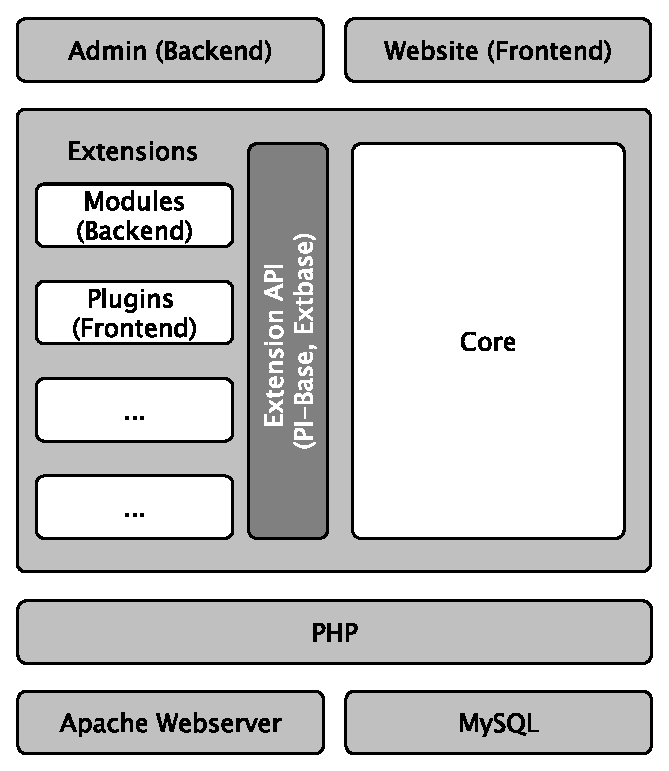
\includegraphics[scale=0.77]{diagrams/TYPO3Architecture.eps}
	\caption{Schematischer Aufbau von TYPO3}
	\label{fig:typo3Architecture}
\end{figure}

Die Gesamtheit aller von TYPO3 CMS zur Verfügung gestellten \gls{api}s, wird als die \mbox{\textit{TYPO3 API}} bezeichnet. Diese kann - analog zum Konzept von Backend und Frontend - in eine \mbox{\textit{Backend \gls{api}}} und eine \mbox{\textit{Frontend \gls{api}}} unterteilt werden. Die Aufgabe der Frontend \gls{api} ist die Zusammenführung der getrennt vorliegenden Bestandteile (Inhalt, Struktur und Layout) aus der Datenbank oder dem Cache zu einer HTML-Seite. Die Backend \gls{api} stellt Funktionen zur Erstellung und Bearbeitung von Inhalten zur Verfügung. (vgl. \cite[S. 5 ff.]{book:dulepovTypo32008})

Die \gls{api}s, die keiner der beiden Kategorien zugeordnet werden kann, bezeichnet Dulepov \cite[S. 5 ff.]{book:dulepovTypo32008} als \mbox{\textit{Common-\gls{api}}}. Die Funktionen der Common-\gls{api} werden von allen anderen \gls{api}s genutzt. Ein Beispiel dafür stellt die Datenbank \gls{api} dar, welche in der Regel nur einfache Funktionen wie das Erstellen, Einfügen, Aktualisieren, Löschen und Leeren\footnote{CRUD - {\bfseries C}reate, {\bfseries R}etrieve, {\bfseries U}pdate und {\bfseries D}elete \label{ft:crud}} von Datensätzen bereitzustellen hat. Auf die aktuelle Datenbank-\gls{api} wird in Kapitel \ref{sec:currentSituation} näher eingegangen.

\subsubsection{XCLASS}
TYPO3 CMS besitzt einen – als XCLASS bezeichneten – Mechanismus, der es erlaubt Klassen zu erweitern oder Methoden mit eigenem Code zu überschreiben. Dies funktioniert für den Systemkern wie auch für andere Extensions. Damit eine Klasse per XCLASS erweiterbar ist, darf sie nicht per \phpinline{new()} Operator erzeugt werden, sondern durch \phpinline{\TYPO3\CMS\Core\Utility\GeneralUtility::makeInstance()}.
Diese Methode sucht im globalen \gls{php}-Array \phpinline{$GLOBALS['TYPO3_CONF_VARS']['SYS']['Objects']} nach angemeldeten Klassen, instanziiert diese und liefert sie anstelle der Originalklasse zurück. Dieses Array dient der Verwaltung der zu überschreibenden Klassen und erfolgt in der Datei \pdf{ext\_localconf.php} innerhalb des Extensionsverzeichnisses.

Der Mechanismus hat jedoch ein paar Einschränkungen:

\begin{itemize}
	\itemsep1pt\parskip0pt\parsep0pt
	\item
		der Code der Originalklasse kann sich ändern. Es ist somit nicht sichergestellt, dass der überschreibende Code weiterhin das macht, wofür er gedacht war
	\item
		XCLASSes funktionieren nicht mit statischen Klassen, statischen Methoden und finalen Klassen
	\item
		eine Originalklasse kann nur einmal per XCLASS überschrieben werden
	\item
		einige Klassen werden sehr früh bei der Initialisierung des Systems instanziiert. Das kann dazu führen, dass Klassen die als Singleton ausgeführt sind, nicht überschrieben werden können oder es kann zu unvorhergesehenen Nebeneffekten kommen.
\end{itemize}

\subsection{Extensions}
Extensions sind funktionale Erweiterungen, die in System-, globale und lokale Extensions unterteilt werden. Sie interagieren mit dem Systemkern über die Extension API und stellen die Möglichkeit dar TYPO3 CMS zu erweitern und anzupassen.

Systemextensions werden mit dem System mitgeliefert und befinden sich ausschließlich im Ordner \pdf{typo3/sysext/}. Sie werden nochmals unterteilt in jene, die für den Betrieb von TYPO3 CMS unabdingbar sind und solche die nicht zwangsläufig installiert sein müssen, jedoch wichtige Funktionen beisteuern.

Neben Systemextensions gibt es globale\footnote{Da globale Extensions nur in bestimmten Szenarien einen Sinn ergeben und in der Realität so gut wie nicht vorkommen, wird von der TYPO3 Community der Begriff "Extension" synonym zum Begriff "lokale Extension" verwendet. Die Arbeit folgt dieser Regelung.} und lokale Extensions. Lokale Extensions werden im Ordner \pdf{typo3conf/ext/} und globale Extensions im Ordner \pdf{typo3/ext} installiert.

\subsubsection{Extension Manager}
Der \gls{em} ist ein \gls{be} Modul, über das die Extensions verwaltet werden können. Es erlaubt die Aktivierung, Deaktivierung, das Herunterladen und das Löschen von Extensions. Darüber hinaus bietet der \gls{em} Möglichkeiten zur detaillierten Anzeige von Informationen über die Extensions wie das Changelog, Angaben zu den Autoren und Ansicht der Dateien der Extension.


%-----------------------------------------------
% Dateiname: Doctrine.tex
% Autor    : Stefano Kowalke <blueduck@gmx.net>
% Lizenz   : BSD
%-----------------------------------------------
\section{Doctrine}
Das Doctrine Projekt besteht aus einer Reihe von PHP-Bibliotheken, die Schnittstellen rund um die Datenbankschicht bereitstellen. Die Konzepte sind beeinflusst von Javas \textit{Hibernate}\footnote{\url{http://hibernate.org/}} (vgl. \cite{web:t3nDoctrine2009}) und dem Entwurfsmuster \textit{Active Record}, welches von Martin Fowler \cite{book:fowlerPatterns2003} vorgestellt wird.

Das Projekt wurde 2006 von Konsta Vesterinen\footnote{\url{http://docs.doctrine-project.org/projects/doctrine1/en/latest/en/manual/acknowledgements.html}} initiiert und im Jahr 2008 als Version 1.0.0 veröffentlicht. Die Version 2.0 wurde im Jahr 2010 unter dem neuen Projektleiter Benjamin Eberlei fertiggestellt.

Die beiden bekanntesten Produkte des Projekts sind:
\begin{itemize}
	\item \gls{orm} - ermöglicht die objekrelationale Abbildung von Objekten auf Datenbanktabellen
	\item \gls{dbal} - stellt eine Datenbankabstraktionsschicht bereit
\end{itemize}

Wie aus Abbildung~\ref{fig:doctrineArchitecture} ersichtlich wird, ist Doctrine DBAL lediglich als eine dünne Schicht auf Basis der \gls{php}-Extension \gls{pdo} ausgeführt, die die grundlegenden Funktionen zur Abstraktion von Datenbanken implementiert. Die ORM Schicht baut auf Doctrine DBAL auf.

\begin{figure}[H]
    \centering
    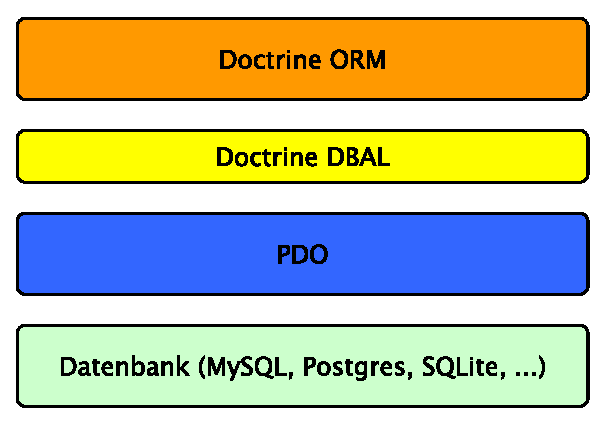
\includegraphics[scale=0.75]{diagrams/DoctrineArchitecture.eps}
    \caption{Schematischer Aufbau von Doctrine}
    \label{fig:doctrineArchitecture}
\end{figure}

\begin{shadequote}[l]{Jonathan Wage \cite{web:t3nDoctrine2009}}
	Ein ORM ist eine Abstraktionsschicht zwischen relationaler Datenbank und der eigentlichen Anwendung. Statt per SQL kann man durch das ORM objektorientiert auf die Daten zugreifen.
\end{shadequote}

Das folgende Anwendungsbeispiel zeigt eine typische Situation. Es wird zunächst ein neues Objekt eines Studenten erzeugt um im weiteren Verlauf mit verschiedenen Daten angreichert. Anschließend wird es als zu speicherndes Objekt bei der Datenbank registiert und schlußendlich gespeichert.

Im zweiten Codelisting wird die gleiche Aufgabe auf dem herkömmlichen Weg gelöst. Dabei wird die Anfrage an eine MySQL und PostgreSQL Datenbank gesendet. Die Variable \phpinline{$connection} enthält je eine initialisierte Verbindung zur entsprechenden Datenbank.

\begin{listing}
\begin{phpcode}
<?php

$student = new Student();
$student->setFirstName('Stefano');
$student->setLastName('Kowalke');
$student->setEnrolmentNumber('12345');
$entityManager->persist($student);
$entityManager->flush();
\end{phpcode}
\caption{Speichern eines Studenten in die Datenbank mit ORM}
\label{lst:orm}
\end{listing}

\begin{listing}
\begin{phpcode}
<?php

$sql =
    'INSERT INTO students ('first_name', 'last_name', 'enrolment_number')
    VALUES ('Stefano', 'Kowalke', '12345');

// MySQLi
$result = mysqli_query($connection, $sql);

// PostgreSQL
$result = pg_query($connection, $sql);

\end{phpcode}
\caption{Speichern eines Studenten in die Datenbank ohne ORM}
\label{lst:withoutOrm}
\end{listing}

Der Code in Listing~\ref{lst:orm} gibt keinen Rückschluss auf die darunterliegende Datenbank. Die Daten des Studenten könnten in eine CSV-Datei, einer MySQL oder Postgres Datenbank gespeichert worden sein. Hingegen wurden in Listing~\ref{lst:withoutOrm} zwei verschiedene Methoden genutzt, um die Daten in eine MySQL und Postgres Datenbank zu schreiben. Die Speicherung in eine Textdatei wurde dabei nicht berücksichtigt.

Doctrine ORM ist für die Umwandlung des \phpinline{$student}-Objekt in eine \gls{sql}-Abfrage zuständig. Die erzeugte Abfrage ist mit der aus Codebeispiel~\ref{lst:withoutOrm} vergleichbar. Die Konvertierung der Anfrage in die verschiedenen \gls{sql}-Dialekte\footnote{Als \gls{sql} Dialekt wird ein vom \gls{sql}-Standard abweichender Hersteller-spezifischer Sprachumfang bezeichnet. Ein Dialekt ist in der Regel kompatibel mit dem Standard und erweitert ihn um eigene Sprachkonstrukte.} erfolgt durch Doctrine DBAL.

Doctrine konvertiert das Schema anhand von sehr unterschiedlichen Merkmalen in das \gls{sql} der jeweilgen \gls{dbms}, die zum Verständnis einen etwas tieferen Einstieg in die Eigenheiten der \gls{dbms} erfordern. Da dies den Umfang der Arbeit überschreitet, wurden markante Beispiele gewählt, die den Sachverhalt verdeutlichen.

Datenbankschemas werden in Doctrine von der Klasse \phpinline{Schema} repräsentiert. Im Beispiel wird zunächst eine Instanz dieser Klasse erstellt und anschließend wird eine neue Tabelle und mehrere Tabellenspalten mit unterschiedlichen Datentypen angelegt. In Zeile 24 wird das Schema in eine \gls{sql}-Abfrage übersetzt. Davor existiert es lediglich als PHP-Objekt bis zum Ende der Laufzeit des Scripts.

Die Variable \phpinline{$myPlatform} enthält die Information über das aktuelle benutzte \gls{dbms}.

\begin{listing}[H]
\begin{phpcode}
<?php

$schema = new \Doctrine\DBAL\Schema\Schema();
$beUsers = $schema->createTable('be_users‘);
$beUsers->addColumn('uid', 'integer',
  array('unsigned' => TRUE, 'notnull' => TRUE, 'autoincrement' => TRUE)
);
$beUsers->addColumn('pid', 'integer',
  array('unsigned' => TRUE, 'default' => '0', 'notnull' => TRUE)
);
$beUsers->addColumn('username', 'string',
  array('length' => 50, 'default' => '', 'notnull' => TRUE)
);
$beUsers->addColumn('password', 'string',
  array('length' => 100, 'default' => '', 'notnull' => TRUE)
);
$beUsers->addColumn('admin', 'boolean',
  array('default' => '0', 'notnull' => TRUE)
);
$beUsers->setPrimaryKey(array('uid'));
$beUsers->addIndex(array('pid'), 'be_users_pid_idx');
$beUsers->addIndex(array('username'), 'be_users_username');

$queries = $schema->toSql($myPlatform);
\end{phpcode}
\caption{Erstellen eines Schemas mit Doctrine}
\label{lst:createSchema}
\end{listing}

Die beiden Listings \ref{lst:mysqlFromSchema} und \ref{lst:pgsqlFromSchema} zeigen den Inhalt von \phpinline{$queries} – einmal für MySQL und für PostgreSQL.

\begin{listing}[H]
\begin{mysqlcode}
// Der Inhalt von $queries für MySQL
CREATE TABLE `be_users` (
	`uid` int(10) unsigned NOT NULL AUTO_INCREMENT,
	`pid` int(10) unsigned NOT NULL DEFAULT '0',
	`username` varchar(50) COLLATE utf8_unicode_ci NOT NULL DEFAULT '',
	`password` varchar(100) COLLATE utf8_unicode_ci NOT NULL DEFAULT '',
	`admin` tinyint(1) NOT NULL DEFAULT '0',
	PRIMARY KEY (`uid`),
	KEY `be_users_pid_idx` (`pid`),
	KEY `be_users_username` (`username`)
) ENGINE=InnoDB AUTO_INCREMENT=2 DEFAULT CHARSET=utf8 COLLATE=utf8_unicode_ci;
\end{mysqlcode}
\caption{Das erstellte Schema als MySQL Anfrage}
\label{lst:mysqlFromSchema}
\end{listing}

\begin{listing}[H]
\begin{psqlcode}
// Der Inhalt von $queries für PostgreSQL
CREATE TABLE be_users (
	uid serial NOT NULL,
	pid integer NOT NULL DEFAULT 0,
	username character varying(50) NOT NULL DEFAULT ''::character varying,
	password character varying(100) NOT NULL DEFAULT ''::character varying,
	admin boolean NOT NULL DEFAULT false,
	CONSTRAINT be_users_pkey PRIMARY KEY (uid)
) WITH (
	OIDS=FALSE
);
\end{psqlcode}
\caption{Das erstellte Schema als PostgreSQL}
\label{lst:pgsqlFromSchema}
\end{listing}

Anhand der Beispiel kann folgendes abgeleitet werden:

\begin{itemize}
	\item die Deklaration von  mit \phpinline{integer ... auto_increment} wird nach \sqlinline{int(10) ... AUTO_INCREMENT} für MySQL und \sqlinline{serial} für PostgreSQL übersetzt
	\item die einfache Deklaration von \phpinline{INTEGER} wird nach \sqlinline{INT(10)} und \sqlinline{INTEGER} übersetzt
	\item \phpinline{string} wird nach \sqlinline{VARCHAR} bzw. \sqlinline{CHARACTER VARYING} übersetzt.
	\item \phpinline{boolean} wird nach \sqlinline{TINYINT(1)} für MySQL und \sqlinline{BOOLEAN} für Postgres übersetzt.
\end{itemize}

Dabei geben die Werte in Klammern die Länge des Datentyps an. Es ist zu beachten, dass die Länge für String-Typen eine andere Bedeutung hat, als für numerische Datentypen. Wird ein \sqlinline{VARCHAR} mit der Länge \textit{34} definiert, bedeutet dies, dass darin eine Zeichenkette mit maximal 34 Zeichen inklusive Leerzeichen gespeichert werden kann. Würde man auf den (vollkommen abwegigen) Gedanken kommen in dieser Spalte das Buch \textit{The Hitchhiker's Guide to the Galaxy} von Douglas Adams speichern zu wollen, würde der Inhalt wie folgt aussehen: ``Far out in the uncharted backwate'' \cite[S. 3]{book:adamsHitchhikers1995}

Bei numerischen Datentypen beschreibt der Wert allerdings die Anzeigenbreite - also die Anzahl der angezeigen Ziffern des gespeicherten Wertes. Sollte der in der Spalte gespeicherte Wert kleiner sein als die Länge der Anzeigenbreite, werden die restlichen Stellen nach links mit Leerzeichen aufgefüllt. Wurde die Option \sqlinline{ZEROFILL} gesetzt, werden die restlichen Stellen mit Nullen anstelle von Leerzeichen aufgefüllt. Der Wert beinflusst in keinster Weise den maximal speicherbaren Wert. In einer als \sqlinline{TINYINT} definierten Spalten können immer 256 Werte gespeichert werden. Unabhängig davon ob sie mit \sqlinline{TINYINT(1)} oder \sqlinline{TINYINT(4)} deklariert wurde.


Hier kann man die Unterschiede der verschiedenen Hersteller erkennen. Die Ursachen liegen darin begründet, dass die verschiedenen Hersteller eigene Features in ihre Datenbanken implementiert haben, oder sich die interne Verwaltung der Daten unterscheidet. Dies ist vergleichbar mit dem HTML-Standard und den Browser-spezifischen Tags. Als Stichwort sei hier SQLite genannt, die die Daten wahlweise in einer Datei oder im RAM speichert und sich somit grundsätzlich von Datenbanken wie MySQL, Postgres oder Oracle unterscheidet, die die Daten in mehren Dateien ablegen.

Datenbanken verwalten die Daten in Datentypen, wie es von typisierten Programmiersprachen wie C und C++ bekannt ist. Jedoch bieten nicht alle Hersteller die gleichen Typen an. So gibt es zum Beispiel keinen \textit{Boolean}-Typ in MySQL; jedoch in Postgres. Doctrines Repräsentation des Datenbankschemas ist generisch ausgestaltet, damit es den angebenen Datentyp in das Datenbank-spezifische Äqvivalent umsetzen kann.


Gibt es mehrere ähnliche Datentypen wie \sqlinline{TINYINT} und \sqlinline{INT} oder \sqlinline{VARCHAR} und \sqlinline{LONGTEXT}, trifft Doctrine die Entscheidung anhand der Länge des Datentyps. Wird keine Länge bei der Schemadeklaration angegeben, wird der Standardwert der jeweiligen Datenbank gewählt.

- Konfus: bit und boolean
- Tinyint = Boolena in MySQL
Als Grundlage der Länge eines Datentypes dient das Binärsystem, in dem es lediglich zwei Werte – 0 und 1 - gibt. Dies erlaubt die Abbildung der Zusände \textit{An} und \textit{Aus} oder \textit{Ja} und \textit{Nein}. Dies entspricht den Datentyp \textit{Boolean}. In der Regel müssen allerdings größere Werte gespeichert werden. Dazu werden acht Bits zu einem Byte zusammengefasst.



Zu beachten sind an diesem Beispiel die folgenden Besonderheiten:
\begin{itemize}
	\item Autoincrement - autoincrement / Serial
	\item Boolean - tinyint / Boolean
	\item string - varchar / charakter varying
	\item primary key - \sqlinline{PRIMARY KEY (`uid`)} / \sqlinline{CONSTRAINT be_users_pkey PRIMARY KEY (uid)}
	\item \phpinline{$beUsers->addIndex} - \sqlinline{KEY `be_users_pid_idx` (`pid`)} / Indices werden in Postgres gesondert verwaltet (Screenshot einfügen)
\end{itemize}

%-----------------------------------------------
% Dateiname: PDO.tex
% Autor    : Stefano Kowalke <blueduck@gmx.net>
% Lizenz   : BSD
%-----------------------------------------------
\section{PDO}
Wie wir im Kapitel über Doctrine sehen werden [Hängt davon ab, wo dieses Kapitel eingefügt wird], baut es auf \gls{pdo} auf. Es verwendet dessen Konzepte und erweitert diese. Um ein tieferes Verständnis von Doctrine \gls{dbal} zu erlangen, kommt man nicht umhin sich mit \gls{pdo} zu beschäftigen.

Im diesem Kapitel wird auf den Hintergrund von \gls{pdo}. Es werden die Fähigkeiten und Grenzen aufgezeigt, sowie anhand von einfachen Beispielen die Funktionsweise illustriert.

\subsection{Was ist PDO}
PHP Data Objects (PDO) stellt eine Abstraktionsbibliothek für die Interaktion mit \gls{dbms} verschiedener Hersteller dar und orientiert sich dabei an dem Konzept der \gls{jdo}\footnote{\url{http://www.oracle.com/technetwork/java/index-jsp-135919.html}}. Es ist seit Version 5.1 in \gls{php} enthalten.

Der Grund der Existenz einer solchen Bibliothek liegt darin begründet, dass man in PHP viele verschiedene \gls{dbms} über jeweils eigene Extensions ansprechen kann. Die dazu extra zu installierenden Extensions bringt jeweils eine eigene API für die \gls{dbms} mit, so das sich die Art des Aufbaues der Verbindung und das Absetzen von Anfragen von \gls{dbms} zu \gls{dbms} unterschiedlich ausgestaltet ist.
Dies kann zu einem hohem Aufwand führen, wenn die Anwendung von einem \gls{dbms} auf ein anderes umgestellt werden soll. \gls{pdo} hingegen definiert unabhängig vom zugrundeliegenden \gls{dbms} eine einheitliche Schnittstelle für das Verbindungsmanagement und die Kommunikation mit der Datenbank.

Neben \gls{pdo} existieren unter anderen die Projekte  MDB2\footnote{\url{http://pear.php.net/package/MDB2}} und ADOdb\footnote{\url{http://adodb.sourceforge.net/}}, die den gleichen Ansatz verfolgen. Wenn man sich jedoch die letzten Releasedaten\footnote{bei MDB2 2.5.0b5 war die letzte Veröffentlichung am 2012-10-29; bei ADOdb am 2012-09-04} beider Projekte ansieht, kann man leicht den Eindruck erhalten, dass sie nicht mehr weiterentwickelt werden.

Ein weiterer Vorteil von \gls{pdo} gegenüber anderen Projekten ist die Geschwindigkeit, da es vollständig in C++ programmiert wurde.

(vgl. \cite[S. 5]{book:popel2007pdo})

\subsection{Limitierungen}
Bei einer Abstraktion wird stets etwas Spezifisches, durch das Weglassen von Details, in etwas Allgemeines überführt. Im Fall von \gls{pdo} wird der andere Weg gegangen – es werden allgemeine \gls{sql}-Anfragen in den Dialekt\footnote{Als Dialekt wird die Hersteller-eigene Implementation des \gls{sql}-Standards genannt, dass sich im Umfang und Syntax vom Standard unterscheidet.} des Herstellers übersetzt.

Aus diesem Grund vermag es \gls{pdo} nicht eine SQL-Abfrage, die in dem Dialekt eines Herstellers formuliert wurde, in den eines anderen zu übersetzen. Stattdessen muss die Anfrage so nah wie möglich am Standard gestellt werden, um als portabel zu gelten.

[Beispiel einfügen SQL-Standard und eigene Erweiterung von MySQL -> Siehe Buch Seite 17]

\subsection{Verwendung}
Der grundlegende Unterschied von PHP-Extensions wie die für MySQL und PosgreSQL zu PDO besteht darin, dass die zuerst genannten eine prozeduale Bibliothek darstellen und \gls{pdo} streng Objekt-orientiert aufgebaut ist. Während diese Extensions lediglich Funktionen zur Interaktion mit der Datenbank zur Verfügung stellen, die keine weiteren Informationen über den inneren Zustand der Verbindung besitzen, führt \gls{pdo} Klassen ein, die sowohl die Verbindung als auch die eine Abfrage kapseln und als Schnittstelle dienen.

Die Klasse \phpinline{PDO} beinhaltet die Verbindung zur Datenbank und stellt Methoden zum Verbindungsmanament bereit, während die Klasse \phpinline{PDOStatement} eine Schnittstelle zu Anfragen und teilweise auch zur Ergebnismenge\footnote{Da alle betrachteten Datenbanken den relationalen Datenbanken zuzuschreiben sind, handelt es sich bei den Datenbanktabellen um die mathematischen Beschreibung einer Relation . Zudem kann eine Relation/Tabelle als eine Menge aufgefasst werden. Verknüpft man Relationen mit Operatoren (Abfrage) erhält man stets wieder eine Relation. Somit ist das Ergebnis einer Abfrage eine Menge - die Ergebnismenge} bietet.%[http://de.wikipedia.org/wiki/Relationale_Datenbank]

Im Folgenden wird die Verwendung der Klassen an einfachen Beispielen erläutert. Dabei werden die Unterschiede zur den klassischen Verfahren (MySQL und PostgreSQL) demonstriert. Damit \gls{pdo} mit verschiedenen \gls{dbms} benutzt werden kann, müssen die Treiber des entsprechenden \gls{dbms} installiert sein. Als Grundlage der Abfragen und Ergebnisse dient eine Datenbank mit den folgenden Tabellen. Es wird davon ausgegangen, dass sie bereits erstellt wurde.

\begin{Verbatim}[samepage=true]
students
+----+------------+-----------+-------+
| id | first_name | last_name | house |
+----+------------+-----------+-------+
|  1 | Lucius     | Malfoy    |   4   |
|  3 | Herminone  | Granger   |   1   |
|  4 | Ronald     | Weasley   |   1   |
|  5 | Luna       | Lovegood  |   3   |
|  6 | Cedric     | Diggory   |   2   |
+----+------------+-----------+-------+

houses
+----+------------+
| id | name       |
+----+------------+
|  1 | Gryffindor |
|  2 | Huffelpuff |
|  3 | Ravenclaw  |
|  4 | Slytherin  |
+----+------------+
\end{Verbatim}

\subsection{Verbindung aufbauen}
Traditionell wird eine Verbindung wie folgt aufgebaut:

\begin{phpcode}
// MySQLi
$connection = mysqli_connect(
    $host,
    $username,
    $password,
    $dbname
);

// PostgreSQL
$connection = pg_connect(
    'host=' . $host .
    ' dbname=' . $dbname .
    ' user=' . $userName .
    ' password=' . $password
);
\end{phpcode}

Dieses Beispiel zeigt, dass MySQLi\footnote{MySQLi bietet sowohl eine prodezuale als auch eine objektorientierte \gls{api} an. Da TYPO3 CMS auschließlich den  prodezualen Ansatz nutzt und sich dieser nahezu mit derAPI von MySQL deckt, sind die Bespiele in prozedualer Form gehalten.} und PostgreSQL zwar einfache Methoden zur Verfügung stellen, diese sich jedoch in der Benutzung voneinander unterscheiden.

Um eine Verbindung mit \gls{pdo} zu etablieren wird der Konstruktor verwendet, welcher ein Objekt vom Typ PDO zurückgibt. Die Signatur des Konstruktors sieht wie folgt aus:

\begin{phpcode}
public PDO::__construct(
  string $dsn
  [, string $username]
  [, string $password]
  [, array $driver_options]
)
\end{phpcode}

Während die Parameter \phpinline{$username} und \phpinline{$password} selbsterklärend sind und über den letzten Parameter \phpinline{$driver_options} Datenbanktreiber-spezifische Einstellungen übergeben werden können, erfordert der erste Parameter eine nähere Beschreibung.

Mit dem Kürzel \phpinline{$dsn} (engl. Data Source Name) ist die Datenquelle gemeint, die in einem bestimmten Format übergeben werden muss. Dabei wird zuerst der Typ des \gls{dbms} angegeben und - getrennt von einem Doppelpunkt - der Datenbank-spezifische Teil.

\begin{phpcode}
// MySQL
$connection = new PDO(
  'mysql:host=$host;dbname=$db',
  $user,
  $pass
);

// PostgreSQL
$connection = new PDO(
  'pgsql:host=$host dbname=$db',
  $user,
  $pass
);
\end{phpcode}

Das in der Variablen \phpinline{$connection} enthaltene Verbindungsobjekt stellt den Ausgangspunkt für alles Weitere dar. Die naheliegendsten Aktionen nach dem Verbindungsaufbau sind das Absetzen einer SQL-Anfrage an die Datenbank und die Ausgabe des Ergebnisses.

\subsection{Datenbankabfragen}
Die als Beispiel dienende Abfrage soll die Nachnamen aller Studierenden in alphabetischer Reihenfolge ausgeben. Die in einer Variablen gespeicherten SQL-Abfrage wird an die Datenbank gesendet und das Ergebnis über eine Schleife ausgegeben. Zunächst wird der althergebrachte Weg gezeigt. Beide PHP-Extensions stellen dafür \phpinline{*_query} Funktionen zur Verfügung, die eine Kennung der Datenbankverbindung zurückgeben. Im Fall eines Fehlers geben sie \phpinline{FALSE} zurück.

\begin{phpcode}
$sql = 'SELECT last_name FROM students ORDER BY last_name';
// For MySQLi:
$result = mysqli_query($connection, $query);
while($row = mysqli_fetch_assoc($result)) {
	echo $row['last_name'] . ' ';
}

// PostgreSQL:
$result = pg_query($query);
while($row = pg_fetch_assoc($result)) {
	echo $row['last_name'] . ' ';
}
\end{phpcode}

Das \gls{pdo}-Objekt bietet dafür die Methode \phpinline{query()} an, die ein Objekt vom Typ\\
\phpinline{PDOStatement} zurückgibt. Dieses implementiert das Interface Traversable und kann somit - analog zu einem Array - in einer Schleife durchlaufen werden. Ein Aufruf von\\
\phpinline{mysqli_result::fetch_assoc} erübrigt sich.

\begin{phpcode}
$sql = 'SELECT last_name FROM students ORDER BY last_name';

$statement = $connection->query($sql);

foreach($statement as $row) {
  echo $row['last_name'] . ' ';
}
\end{phpcode}

Die Ausgabe aller Bespiele lautet:
\begin{Verbatim}
Diggory Granger Lovegood Malfoy Weasly
\end{Verbatim}

Um das Ergebnis der Abfrage sinnvoll nutzen zu können, gibt es verschiedene Stile (engl. fetch styles) in die es formatiert werden kann. Um dennoch die interne Struktur der Ergebnismenge beinflussen zu können, gibt es in \gls{pdo} Konstanten, die als optionales Argument an \phpinline{query()} übergeben werden. In der Defaulteinstellung benutzt \gls{pdo} die Konstante \phpinline{PDO::FETCH_BOTH}, bei dem das Ergebnis zum einen über den Spaltenbezeichner (wie im obigen Beispiel) als auch über eine Indexzahl angesprochen werden kann. Im Beispiel würde das so aussehen: \phpinline{echo $row[0]}.

Zu allen \phpinline{*_fetch_*}-Methoden gibt es das entsprechende Äquivalent als \gls{pdo}-Konstante. Die Wichtigsten sind:

\begin{itemize}
	\item \phpinline{PDO::FETCH_ASSOC} - entspricht \phpinline{*_fetch_assoc()}
	\item \phpinline{PDO::FETCH_NUM} - entspricht \phpinline{*_fetch_array()}
	\item \phpinline{PDO::FETCH_ROW} - entspricht \phpinline{*_fetch_row()}
\end{itemize}

Darüberhinaus definiert \gls{pdo} noch weitere Konstanten, die keine Ensprechungen haben.

\begin{itemize}
	\item \phpinline{PDO::FETCH_OBJ} - liefert jede Zeile der Ergebnisrelation als Objekt zurück. Die Spaltenbezeichner werden dabei zu Eigenschaften der Klasse.
	\item \phpinline{PDO::FETCH_LAZY} - wie \phpinline{PDO::FETCH_OBJ}. Das Objekt wird jedoch erst dann erstellt, wenn darauf zugegriffen wird.
	\item \phpinline{PDO::FETCH_CLASS} - liefert eine neue Instanz der angeforderten Klasse zurück. Die Spaltenbezeichner werden dabei zu Eigenschaften der Klasse.
	\item \phpinline{PDO::FETCH_COLUMN} - liefert nur eine Spalte aus der Ergebnismenge zurück.
\end{itemize}

Dies stellt eine nicht abschließende Aufzählung dar. Die Dokumentation von \gls{pdo} benennt weitere sogenannte \textit{Fetch Styles}-Konstanten\footnote{\url{http://mx2.php.net/manual/en/pdo.constants.php}}, die für diese Arbeit jedoch nicht von Interesse sind.
Die Benutzung der Konstanten erfolgt per Übergabe als Parameter an die \phpinline{query()}-Methode:

\begin{phpcode}
$statement = $connection->query($sql, PDO::FETCH_NUM);

foreach($statement as $row) {
  echo $row[0];
}
\end{phpcode}

Über das \phpinline{PDOStatement}\footnote{Leider ist der Begriff dieser Klasse etwas unglücklich gewählt oder es ist ein Designfehler von \gls{pdo}, denn ein Objekt dieser Klasse repräsentiert zum einen ein (Prepared) Statement und, nachdem die Anfrage ausgeführt wurde, die Ergebnisrelation. Die Methoden der Klasse agieren somit einmal auf dem Statement und einmal auf dem Ergebnis.} werden weitere Möglichkeiten wie die Methoden \phpinline{fetch()} und \phpinline{fetchAll()} angeboten, um das Ergebnis zu erhalten. Diese Methoden müssen auch genutzt werden, wenn statt der \phpinline{foreach}-Schleife eine \phpinline{while}-Schleife genutzt werden soll:

\begin{phpcode}
$statement = $connection->query($sql);

while($row = $statement->fetch(PDO::FETCH_ASSOC)) {
  echo $row['last_name'];
}
\end{phpcode}

Zudem gibt es mit \phpinline{fetch_column()} und \phpinline{fetch_Object()} Alternativen für die Verwendung von \phpinline{fetch()} in Verbindung mit den entsprechenden Konstanten.

\subsection{Prepared Statements}
Bereits MySQLi führt Prepared Statements ein, somit sind sie in der PHP-Welt nicht so neu. Während MySQLi nur einen Typ von Prepared Statements unterstützt, bietet \gls{pdo} eine weitere sinnvolle Variante an. Im Folgenden wird das Konzept und der Nutzen von Prepared Statements kurz erklärt.

Prepared Statements können als eine Vorlage für SQL-Abfragen verstanden werden, die immer wieder, mit verschiedenen Werten, ausgeführt werden. Dabei kann ein \gls{dbms} die Struktur dieses Templates einmalig analyisieren und vorkompiliert im Cache speichern. Bei jedem erneuten Aufruf setzt es lediglich die anderen Werte anstelle von Platzhaltern ein, was die Ausführung schneller macht. (vgl. \cite[S. 75]{book:popel2007pdo})

Zur Demonstration soll je ein Codebeispiel dienen. Dabei fügen wir neue Studierende in die oben gezeigte Datenbanktabelle ein. Der sprechende Hut\footnote{\url{http://de.harry-potter.wikia.com/wiki/Sprechender_Hut}} hat bereits über die Häuser der Neuzugänge entschieden. Um die Abfrage einfach zu halten, wird der Fremdschlüssel der Tabelle für die Häuser direkt in dem Query angegeben.

Die Daten der Studierenden liegen in einem assoziativen Array vor und können somit über eine For-Schleife durchiteriert werden. Pro Schleifendurchlauf wird ein Studierender der Datenbank hinzugefügt. Die Werte werden mit der \phpinline{pdo::quote()}-Methode maskiert um SQL-Injections\footnote{SQL-Injections werden im Kapitel \ref{subsec:sqlInjections} behandelt.\label{ftn:maskQueries}} zu unterbinden.

\begin{phpcode}
$students = array (
	array (
		'last_name' => 'Ellesmere',
		'first_name' => 'Corin',
		'house' => 1
	),
	array (
		'last_name' => 'Tugwood',
		'first_name' => 'Havelock',
		'house' => 4
	),
	array (
		'last_name' => 'Fenetre',
		'first_name' => 'Valentine',
		'house' => 3
	)
)

foreach ($students as $student) {
	$sql = 'INSERT INTO students (last_name, first_name, house)
	  VALUES (' . $connection->quote($student['last_name']) .
	    ',' . $connection->quote($student['first_name']) .
	    ',' . $connection->quote($student['house']) . ')');

	$connection->query($sql);
}
\end{phpcode}

Bei jedem Durchlauf wird eine neue Abfrage mit den aktuellen Daten erzeugt und an die Datenbank geschickt. In diesen Fall bietet sich die Benutzung von Prepared Statements an, da sich pro Iteration lediglich die Werte ändern.

\begin{phpcode}
$statement = $connection->prepare(
  'INSERT INTO students (last_name, first_name, house)
    VALUES (?, ?, ?)');

foreach ($students as $student) {
	$statement->execute(
	  array(
	    $student['last_name'],
	    $student['first_name'],
	    $student['house']);
	);
}
\end{phpcode}

Die hier, anstelle der eigentlichen Daten, verwendeten Fragezeichen stellen Platzhalter dar, die als \textit{Positional Placeholders} (engl. Positions Platzhalter) bezeichnet werden. Die Daten werden der Methode \phpinline{PDOStatement::execute()} in einem Array übergeben. Dabei ist die Reihenfolge wichtig, da ansonsten die Daten in die falschen Spalten der Tabelle geschrieben werden.

Bei der Benutzung von Prepared Statements kann auf die Maskierung per \phpinline{PDO::quote()} verzichtet werden, da dies die Datenbank übernimmt.

\gls{pdo} bietet - im Gegensatz zu MySQLi - mit den \textit{Named Paramentern} noch eine weitere Möglichkeit für Platzhalter an. Anstelle von Fragezeichen werden Bezeichner mit einem vorangestellen Doppelpunkt verwendet. Der Vorteil von dieser Variante, dass die Reihenfolge bei der Übergabe der Daten an die \phpinline{PDOStatement::execute()}-Methode keine Rolle mehr spielt. Das folgende Listing zeigt den gleichen Code von oben jedoch diesmal mit Named Parametern. Die Daten werden dieses Mal als Key/Value-Paar übergeben, bei dem der Key den benannten Platzhalter darstellt und der Value die einzufügenden Daten.

\begin{phpcode}
$statement = $connection->prepare(
  'INSERT INTO students (last_name, first_name, house)
    VALUES (:lastname, :firstname, :house)');

foreach ($students as $student) {
	$statement->execute(
	  array(
	    ':firstname' => $student['first_name'],
	    ':lastname'  => $student['last_name'],
	    ':house'     => $student['house']);
	);
}
\end{phpcode}

Nun spielt die Reihenfolge keine Rolle mehr – die Daten werden in die richtige Spalten eingefügt.

Die Zuordnung einer Variablen zu einem Platzhalter wird \textit{Binding} genannt; gebundene Variablen werden demzufolge als \textit{Bounded Variables} bezeichnet. Neben der gezeigten Bindung über\\
\phpinline{PDOStatement::execute()} bietet \gls{pdo} spezialisiserte Methoden an, was folgende Ursachen hat:

\begin{enumerate}
	\item Bei der gezeigten Bindung werden die Variablen stets als String behandelt. Es ist nicht möglich dem \gls{dbms} mitzuteilen, das der übergebene Wert einem anderen Datentyp entspricht.
	\item Die Variablen werden bei dieser Methode stets als In-Parameter übergeben. Auf den Wert der Variablen kann innerhalb der Funktion nur lesenend zugegiffen werden. Man nennt diese Übergabe auch \textit{by Value}. Es gibt jedoch Szenarien in denen der Wert der Variable innerhalb der Funktion geändert werden soll. Dann müssen die Parameter als Referenz (\textit{by Reference}) übergeben werden und agieren als In/Out-Paramaeter. Einige \gls{dbms} unterstützen dieses Vorgehen und speichern das Ergebnis der Abfrage wieder in der übergebenen Variable.
\end{enumerate}

Das Äquivalent zum obigen Beispiel ist die Methode \phpinline{PDOStatement::bindValue()}, bei der die Variable als In-Parameter übergeben wird. Für jeden zu bindenden Platzhalter muß die Methode aufgerufen werden, die den Name des Platzhalters, den zu bindenen Wert und die optionale Angabe des Datentyps erwartet. \gls{pdo} bietet dazu vordefinierte Konstanten an, die den \gls{sql} Datentypen entsprechen.

\begin{phpcode}
$statement = $connection->prepare(
  'INSERT INTO students (last_name, first_name, house)
    VALUES (:lastname, :firstname, :house)');

foreach ($students as $student) {
    $statement->bindValue(':lastname', $student['first_name']);
    $statement->bindValue(':firstname', $student['last_name']);
    $statement->bindValue(':house', $student['house'], PDO::PARAM_INT);

	$statement->execute();
}
\end{phpcode}

Die Methode zur Übergabe der zu bindenden Werte per Referenz heißt \phpinline{PDOStatement::bindParam()}. Die Funktionsweise unterscheidet sich dahingehend von \phpinline{bindValue()}, als dass die Werte, welche in der Variablen gespeichert sind, erst dann aus der Adresse im Speicher ausgelesen werden, wenn \phpinline{execute()} ausgeführt wird, während \phpinline{bindValue()} die Werte sofort bei Aufruf der Funktion ausliest. Aus diesem Grund muß \phpinline{bindValue()} innerhalb der Schleife stehen.

\begin{phpcode}
$statement = $connection->prepare(
  'INSERT INTO students (last_name, first_name, house)
    VALUES (:lastname, :firstname, :house)');

$statement->bindParam(':lastname', $student['first_name']);
$statement->bindParam(':firstname', $student['last_name']);
$statement->bindParam(':house', $student['house'], PDO::PARAM_INT);

foreach ($students as $student) {
	$statement->execute();
}
\end{phpcode}


\subsection{SQL-Injections}
\label{subsec:sqlInjections}
[SQL injections Mummy image einfügen]

Bei SQL-Injections kann über das Frontend einer Anwendung eine Zeichenkette in eine SQL-Abfrage injiziert werden, die die Fähigkeit besitzt den betroffenen SQL-Code derart zu verändern, dass er

\begin{itemize}
	\item Informationen wie den Adminbenutzer der Webanwendung zurückliefert
	\item Daten in der Datenbank manipuliert um ein neuer Adminbenutzer anzugelegen
	\item oder die Datenbank ganz- oder teilweise löscht
\end{itemize}

Für ein kurzes Beispiel einer SQL-Injection soll ein Formular dienen, indem nach den Nachnamen der Studierenden aus Hogwarts gesucht werden kann. Der gesuchte  Datensatz wird ausgegeben wenn er gefungen wird, ansonsten erscheint eine entsprechende Meldung. Der in das Inputfeld eingegebene Wert wird von PHP automatisch in der Variablen \phpinline{$_REQUEST} gespeichert und kann in der Anwendung ausgelesen werden. \phpinline{'SELECT * FROM students WHERE last_name = Diggory'} stellt eine mögliche, zu erwartende SQL-Anfrage dar.

[Balsamico Formular einfügen]

\begin{phpcode}
$sql = "SELECT * FROM students
  WHERE last_name = '" . $_REQUEST['lastName'] . "'";

$statement = $connection->query($sql);

foreach($statement as $student) {
  echo 'Lastname: ' . $student['last_name'] . "\n";
  echo 'Firstname: ' . $student['first_name'] . "\n";
  echo 'Haus: ' . $student['house'] . "\n";
}
\end{phpcode}

Dieser Code beinhaltet zwei Fehler:

\begin{enumerate}
	\item Es wird nicht überprüft, ob \phpinline{$_REQUEST['lastName']} leer ist oder was ganz anders enthält als erwartet.
	\item die Benutzereingabe wird nicht maskiert
\end{enumerate}

Im Falle einer leeren Variable, sähe die Abfrage so aus: \phpinline{'SELECT * FROM students WHERE last_name = '}. Im besten Fall gibt sie eine leere Ergebnismenge zurück im schlechtesten einen Fehler. Diese Problem ist leicht zu lösen, indem zum einen auf die Existenz der Variablen geprüft wird und zum anderen ob sie einen Wert enthält. Zusätzlich sollte noch auf den Datentyp des enthaltenen Wertes geprüft werden. Erst dann wird die Anfrage abgesetzt.

Da die Eingabe nicht maskiert wird, interpretiert der SQL-Parser einige Zeichen als Teil als Steuerzeichen der SQL-Syntax. Beispiele solcher Zeichen sind das Semikolon, der Apostroph und ein Backslash.

Selbst ein Websitebesucher ohne böse Ansichten könnte mit der Suche nach einem Studenten mit dem Namen O'Hara die SQL-Injection auslösen. Die in diesen Fall an die Datenbank gesendetet SQL-Anfrage \phpinline{'SELECT * FROM students WHERE last_name = 'O'Hara';} würde wohl einen Fehler auslösen, da der Parser die Anfrage nach dem \textit{O} anhand des Apostroph als beendet interpretiert und \textit{Hara} kein gültiges Sprachkonstrukt von SQL darstellt.

Ein Angreifer könnte hingegen die Eingabe in das Formular nach \phpinline{' or '1'='1} verändern. Damit würde sich diese Abfrage \phpinline{'SELECT * FROM students WHERE last_name = '' or '1'='1';} ergeben.

Wird die Maskierung mit einer entsprechenden Prüfung von Benutzereingaben kombinert, verhindert das die Gefahr von SQL-Injections – eine richtige Anwendung vorrausgesetzt. Wie in Fußnote \footref{ftn:maskQueries} bereits erwähnt wurde, müssen an \phpinline{pdo::query()} übergebene SQL-Anfragen mit \phpinline{PDO::quote()} maskiert werden. Traditionell wird dafür die PHP-Methode \phpinline{addslashes()} oder die jeweiligen Maskierungsmethoden der \gls{dbms} verwendet. Für MySQLi wird \phpinline{mysqli_real_escape_string()} verwendet.

Werden Prepared Statements genutzt, müssen die Benutzereingaben trotzdem überprüft, jedoch nicht mehr maskiert werden. Dies übernimmt dann die Datenbank. Wird dem Prepared Statement noch der Typ des Wertes mitgeteilt, kann das \gls{dbms} eine Typprüfung vornehmen und ggf. einen Fehler zurückgeben.


%-----------------------------------------------
% Dateiname: Workstyle.tex
% Autor    : Stefano Kowalke <blueduck@gmx.net>
% Lizenz   : BSD
%-----------------------------------------------
\section{Arbeitsweise}
\label{sec:workstyle}
Aufgrund seiner Aufgabe stellt der Protoyp einen tiefen Eingriff in die Architektur von TYPO3 dar. Vor diesem Hintergrund ist es umungänglich, dass er alle Anforderungen erfüllt, die an eine Systemextension gestellt werden, auch wenn er keine Systemextension ist.

Dies fängt mit der Einhaltung der TYPO3 Coding Guidelines an, geht über die Versionierung des Codes hin zum Einbinden in das TYPO3 Testframework

\subsection{Formatierung des Quellcodes}
Programmier neigen zu unterschiedlichen Programmierstilen, was solange kein Problem darstellt, solange sie allein an einem Projekt arbeiten. Kommen mehr Entwickler hinzu und es vermischen sich verschiedene Stile, kann es schnell unübersichtlich werden. Um den Sinn eines Programms zu verstehen, hilft es allmein, wenn die Codebasis in einer konsistenten Form formatiert wurde. Dies erhöht die Wartbarkeit und verbessert die Code Qualität.

Coding Guidelines stellen dabei das Regelwerk dar auf das sich die Entwickler eines Projekts geeingt haben.

In den TYPO3 Coding Guidelines (CGL)\footnote{\url{http://docs.typo3.org/typo3cms/CodingGuidelinesReference/6.2/_pdf/manual.t3cgl-6.2.pdf}} wird die Verzeichnisstruktur von TYPO3 selbst, sowie die von Extensions erläutert. Sie erklären die Namenskonventionen für Dateien, Klassen, Methoden und Variablen und beschreiben den Aufbau einer Klassendatei mit notwendigen Inhalt, der unabhängig von dem Zweck der Klasse vorhanden sein muss.

Der größter Teil der CGL behandelt die Formatierung verschiedene Sprachkonstrukte wie Schleifen, Arrays und Bedingungen.

Da das Regelwerk mit 28 Seiten recht umfangreich aussfällt, wird zur Überprüfung des Quellcodes das Programm PHP\_CodeSniffer\footnote{\url{https://github.com/squizlabs/PHP_CodeSniffer}} in Zusammenhang mit dem entsprechendem Regelset für das TYPO3 Projekt \footnote{\url{https://github.com/typo3-ci/TYPO3CMS}} verwendet.

\subsection{Unit Testing}
Eine Anforderung an den Prototyp war, dass er die alte Datenbank API weiterhin unterstützt. Dadurch ist gewährleistet, dass noch nicht angepasste Extensions weiterhin funktionieren. Um dies zu überprüfen muß die Funktionaliät von TYPO3 in Verbindung alter API / neue API fortlaufend getestet werden.

Ein möglicher Ansatz wäre es, mit zwei identischen TYPO3 Installationen zu starten, die mit der Zeit auseinander divergieren, indem eine der beiden APIs immer mehr auf die neue API umgebaut würde. Das Testen dabei kann jedoch nur auf eine stichprobenartige Überprüfung der Funktionaliät des manipulierten Systems beruhen, da es nahezu unmöglich ist, durch dieses manuelle Vorgehen alle Testfälle abzudecken.

Ein andere Ansatz würde auf der Code Ebene ansetzen und pro Methode der alten API verschiedene Testfälle definieren, welche nachvollziehbar wären und immer wieder ausgeführt werden könnten.

Das dafür in Frage kommende Framework heißt PHPUnit\footnote{\url{http://phpunit.de/}}. Es stellt das PHP Pedant von dem aus der Javawelt bekannten JUnit dar und wird von TYPO3 unterstützt. TYPO3 bringt selbst schon über 6000 UnitTests mit\footnote{\url{https://travis-ci.org/TYPO3/TYPO3.CMS/builds/23070563}}.

Das eingangs umrissene Szenario stellt lediglich ein greifbares Beispiel für den Nutzen von Unit Tests dar und ist keineswegs auf Spezialfälle wie Refactorings oder dem Austausch einer API beschränkt. In der vorliegenden Arbeit wurden alle implementierten Methoden der neuen API mit Unit Tests – in Verbindung mit PHPUnit – abgedeckt.

\subsection{Versionsverwaltung}
Als Versionsverwaltung wurde GIT\footnote{\url{http://git-scm.com/}} in Verbindung mit dem Code Hostingdienst GiHub\footnote{\url{http://github.com}} genutzt. Github dient zum einen als Backup im Falle eines Festplattenausfalls und zum anderen als späterer Anlaufpunkt der Extension für Interessierte.

Ferner hat sich um GitHub eine Vielzahl von Services entwickelt, welche unter anderen dabei hilft, die CodeQualität zu analysieren. Die zwei zu erwähnenden Projekte sind Travis\footnote{LINK} und Scrutinizer\footnote{LINK}, welche für das Projekt genutzt wurden.

\subsection{Travis-CI}
Travis-CI ist ein \textit{Continuous Integration} (CI) Service, welcher auf Github gehostete baut.

Der Begriff "bauen" kommt von Sprachen wie C oder Java, die erst kompiliert werden müssen (engl. to compile oder to build), bevor sie ein ausführbares Programm darstellen. Im Gegesatz zu interpretierten Sprachen, die zur Laufzeit von einem Interpreter übersetzt werden. Hier definiert der Begriff "bauen" im Zusammmenhang mit CI das auschecken des Codes aus einem Repository und die Ausführung von:

	\begin{itemize}
		\item Tests (Unit-, Smoke-, Akteptanz- und Behaviortests),
		\item statischer Codeanalysen wie den oben genannten PHP\_CodeSniffer, PHPDepend\footnote{\url{http://pdepend.org/}}, PHP Mess Detection\footnote{\url{http://phpmd.org/}} oder PHP Copy and Paste\footnote{\url{https://github.com/sebastianbergmann/phpcpd}}
	\end{itemize}

Die Konfiguration von Travis-CI erfolgt über eine Textdatei im YAML-Format\footnote{\url{http://www.yaml.org/start.html}} und liegt im Wurzelverzeichnis des Projekts.

[Beispiel einer YAML Datei für Travis einfügen]

Da der Prototyp aus zwei Teilen besteht, wurden zwei Travisprojekte erstellt. Eins für die Extension und eins für den modifizierten TYPO3 Kern.

\subsubsection{Konfiguration für die Extension}
PHPUnit
CodeSniffer
PHPCPD
PHPMessDetection
PHPLOC

Ziel war eine möglichst 100\% Testabdeckung zu erreichen.

\subsubsection{Konfiguration für den TYPO3 Kern}
Während bei den Tests der Extension auf eine innere Konsistenz des Programmcodes geschaut wurde, wurde bei den Tests des Kerns Augenmerk auf die Integration der Extension in das modifizierte TYPO3 gelegt. Ziel war es, dass alle mitgelieferten Tests des Cores erfüllt werden.

\subsection{Scrutinizer}
[Bild einfügen]
Es kann zweifelsfrei gesagt werden, dass Travis-CI das Arbeitstier ist. Außer den oben beschriebenen Tätigkeiten macht er nicht viel. Das Besondere daran ist jedoch, dass er diese Aufgaben unermüdlich mit der gleichen Gewissenhaft ausführt. Das ist die Stärke eines solchen Progamms. Am Ende steht jedoch immer nur ein binäres Ergebnis:

* die Tests sind bestanden
* es sind Tests fehlgeschlagen

Anhand dieses Ergebnis können dann weitere Entscheidungen getroffen werden. Zum Beispiel wird es sinnvoll sein bei einem negativen Ergebnis darauf zu verzichten ein Download Paket zu erstellen und veröffentlichen.

Braucht man jedoch eine graphische Auswertung, der durch die statische Codeanalysen gewonnen Daten, kommt ein Service wie Scrutinizer zum Einsatz. Wie schon bei Travis-CI erfolgt die Konfiguration über eine YAML Datei.

Wie Tests gezeigt haben\footnote{\url{https://scrutinizer-ci.com/g/Konafets/TYPO3v4-Core/inspections}} ist es gegenwärtig nicht möglich den TYPO3 Kern mit Scrutinizer auszuwerten, da das Tool verschiedene Limits implementiert hat. Dies Limits werden von TYPO3 teilweise um ein Vielfaches überschritten. Es ist lediglich gelungen die Auswertung der Analyse zum Umfang des Codes und zur Copy and Paste Detection darzustellen. Da dies jedoch keine ausreichende Aussage über die Code Qualität treffen kann und die Qualität des Codes des TYPO3 Kerns nicht im Fokus dieser Arbeit liegt, wurde auf die Auswertung verzichtet.

Es wurde lediglich ein Srcutinizer Projekt für die Extension erstellt.

[Auswertung des Scrutinzer beschreiben]

Eins wird bei 10.000 Issues\footnote{Mit Issues sind Stellen gemeint, die laut Scrutinizer überarbeitet werden müssten} überschritten, welches von fast alles Analysen übertroffen wird. Zum Beispiel und zum anderen hat es einen zeitlichen Timeout, der bei der Analyse der Ergebnisse wie zum Beispiel der Code Coverage\footnote{Abdeckung der Codebasis mit Unit Tests} überschritten wird.

Der Grund für die Verbindung mit Scrutinizer war auch hier der Gedanke an die spätere Veröffentlichung der Extension und stellt die Grundsteinlegung für eine gleichbeleibend hohe Codequalität dar, die überprüfbar sein soll.

\subsection{IDE}
Als Editor wurde die \gls{ide} PHPStorm verwendet, die über Autovervollständig von Variablen, Methoden und Klassen, unterstützt den Programmierer bei der Erstellung von Klassen durch Templates und bietet vielseitige Integration von externen Programmen.

So ist es zum Beispiel möglich die PHPUnit Tests von PHPStorm aus zu starten und mit ein wenig Konfiguraton \cite{web:kowalke14} kann man sich die CodeCoverage im Editor anzeigen lassen.

Die PHPStorm verfügt über einen Debug Listener, der auf ein vom Browser gesendetes Token wartet und bei Empfang den Debug Prozess startet. Für den verwendeten Browser \textit{Chrome} ist ein Addon verfügbar, mittels diesem das Senden des Debug-Tokens per Knopfdruck ein- und ausgeschaltet werden kann.

Wird der Browser und die \gls{ide} in den Debug-Modus gesetzt und TYPO3 CMS neugeladen, bleibt das Programm an dem gesetzten Breakpoint stehen.


%\section{Ausgangssituation}



		%-----------------------------------------------
% Dateiname: CurrentSituation.tex
% Autor    : Stefano Kowalke <blueduck@gmx.net>
% Lizenz   : BSD
%-----------------------------------------------
\chapter{Aktuelle Situation}
\label{sec:currentSituation}
\section{Die native Datenbank API}
n Kapitel~\ref{basics:typo3:subsubsec:coreAndApi} wurde bereits darauf hingewiesen, dass die einheitliche Datenbank API von der Klasse \phpinline{\TYPO3\CMS\Core\Database\DatabaseConnection} bereitgestellt wird. Über die globale Variable \phpinline{$GLOBALS['TYPO3_DB']} kann darauf zugegriffen werden.

\begin{listing}[H]
	\begin{phpcode}
$GLOBALS['TYPO3_DB']->exec_UPDATEquery(
  $this->user_table,
  $this->userid_column . '=' .
    $this->db->fullQuoteStr(
      $tempuser[$this->userid_column],
      $this->user_table
    ),
  array($this->lastLogin_column => $GLOBALS['EXEC_TIME'])
);

	\end{phpcode}
	\caption{Aktualisierung des Zeitpunkts des letzten Logins}
	\label{lst:databaseOldExample}
\end{listing}

Durch die Nutzung der Datenbank API wird zum einen die Integrität der Daten sichergestellt und es werden die \gls{php}-Datenbankfunktionen abstrahiert. Somit kann die Implementation der API-Methoden angepasst werden, ohne die API selbst zu verändern. Auf diese Weise wurde die Umstellung von MySQL auf die MySQLi durchgeführt.\footnote{\url{http://bit.ly/typo3cms-switch-from-mysql-to-mysqli}}

Die Datenbank API bietet eine Vielzahl an Methoden, die sich in die folgenden fünf Gruppen einteilen lassen:

\begin{enumerate}
	\item Methoden die SQL-Abfragen generieren
	\item Methoden die SQL-Abfragen gegen die Datenbank ausführen
	\item Methoden die auf der Ergebnismenge agieren
	\item Administrative Methoden
	\item Hilfsmethoden
\end{enumerate}

\newpage

\subsection{Generierende Methoden}

Die erste Gruppe besteht aus Methoden, die anhand der übergebenen Parameter einen SQL-Abfrage generieren. Damit werden die typischen CRUD-Operationen~\ref{ft:crud} abgebildet.

\begin{figure}[H]
	\centering
	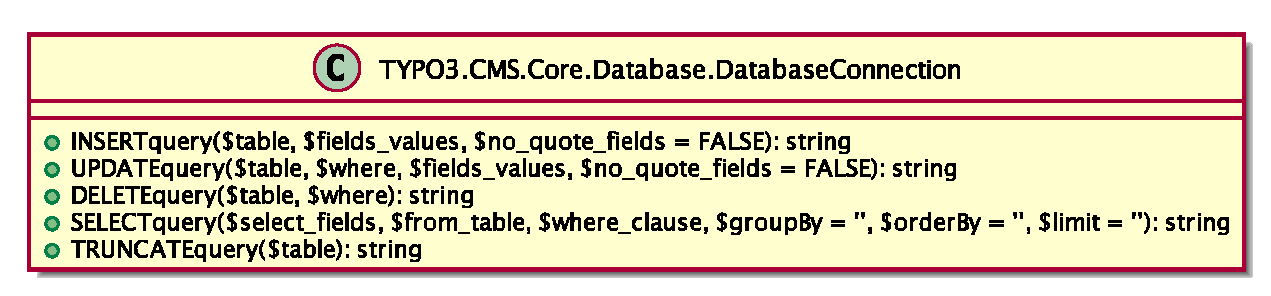
\includegraphics[scale=0.65]{gfx/uml/DatabaseConnectionCreationMethods.eps}
	\caption{Methoden zum Erzeugen von SQL-Abfragen}
	\label{fig:databaseConnectionWithSQLGenerationMethods}
\end{figure}

Folgendes Codebeispiel aus \phpinline{\TYPO3\CMS\Core\Authentication\AbstractUserAuthentication} zeigt die Funktionsweise von \phpinline{SELECTquery()}. Der Kommentar zeigt die generierte SQL-Abfrage.

\begin{listing}[H]
	\begin{phpcode}
// DELETE FROM sys_file_reference WHERE tablenames='pages';
$deleteQuery = $GLOBALS['TYPO3_DB']->DELETEquery(
    'sys_file_reference',
    'tablenames=' . $GLOBALS['TYPO3_DB']->fullQuoteStr(
      'pages',
      'sys_file_reference'
    )
);
	\end{phpcode}
	\caption{Löschen eines Datensatzes aus einer Tabelle}
	\label{lst:databaseOldDeleteExample}
\end{listing}

\subsection{Ausführende Methoden}
Eine Ebene höher setzt die nächste Gruppe an, die die eben gezeigten Methoden nutzt, den generierten SQL-Abfrage ausführt und eine Ergebnismenge vom Typ \phpinline{mysqli_result} zurückliefert.

\begin{figure}[H]
\centering
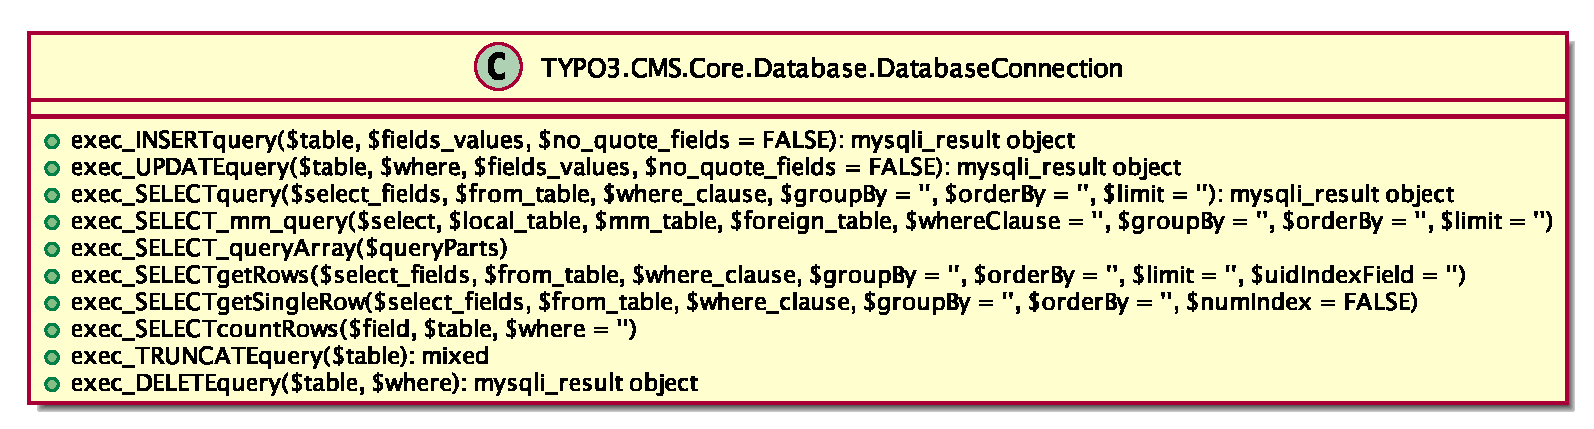
\includegraphics[scale=0.5]{gfx/uml/DatabaseConnectionExecuteMethods.eps}
\caption{Methoden zum Ausführen von SQL-Abfragen}
\label{fig:databaseConnectionWithSQLExecutionMethods}
\end{figure}

\newpage
\subsection{Methoden zur Manipulation der Ergebnismenge}
In der dritten Gruppe befinden sich die Methoden, die im weitesten Sinn zur Verarbeitung der Ergebnismenge genutzt werden. Darunter fallen

\begin{itemize}
	\item jene, die die Daten aus der Ergebnismenge extrahieren,
	\item die für die Fehlerbehandlung genutzt werden können,
	\item sowie Methoden, die Informationen über die Ergebnismenge bereitstellen
\end{itemize}

\begin{figure}[H]
\centering
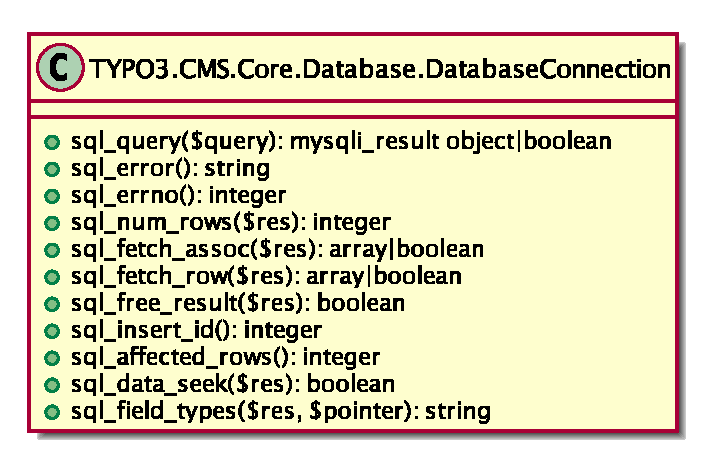
\includegraphics[scale=0.65]{gfx/uml/DatabaseConnectionFetchMethods.eps}
\caption{Methoden zur Verarbeitung der Ergebnismenge}
\label{fig:databaseConnectionWithResultsetsMethods}
\end{figure}


\subsection{Administrative Methoden}
Die nächste Gruppe besteht aus einer Reihe von Methoden, die verschiedene Metadaten über die Datenbank zur Verfügung stellen. Der Name impliziert, dass sie für Administrative Tätigkeiten genutzt werden, was jedoch irreführend ist. Sie werden hauptsächlich während der Installation vom \textit{Installation Tool} verwendet, um Informationen über die zugrundeliegende Datenbank zu erhalten

\begin{figure}[H]
\centering
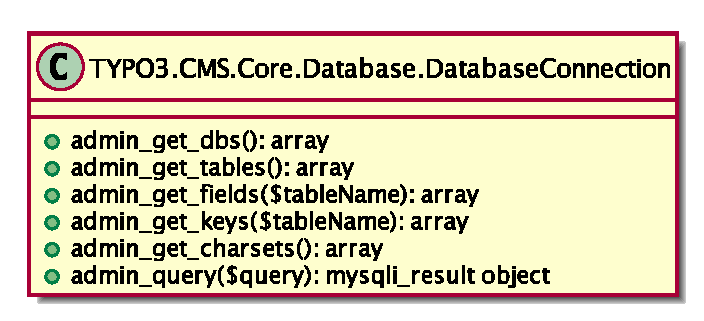
\includegraphics[scale=0.7]{gfx/uml/DatabaseConnectionAdminMethods.eps}
\caption{Administrativen Methoden}
\label{fig:databaseConnectionWithSQLAdminMethods}
\end{figure}

\newpage
\subsection{Hilfsmethoden}
Die letzte Gruppe besteht  aus Hilfsmethoden, die genutzt werden um

\begin{itemize}
	\item einen SQL-Abfrage an die Datenbank zu senden
	\item Benutzereingaben zu maskieren
	\item Listen von Integern zu normalisieren
	\item eine \phpinline{WHERE}-Bedingung aus Komma-separierten Datensätzen zu erzeugen
\end{itemize}

\begin{figure}[H]
\centering
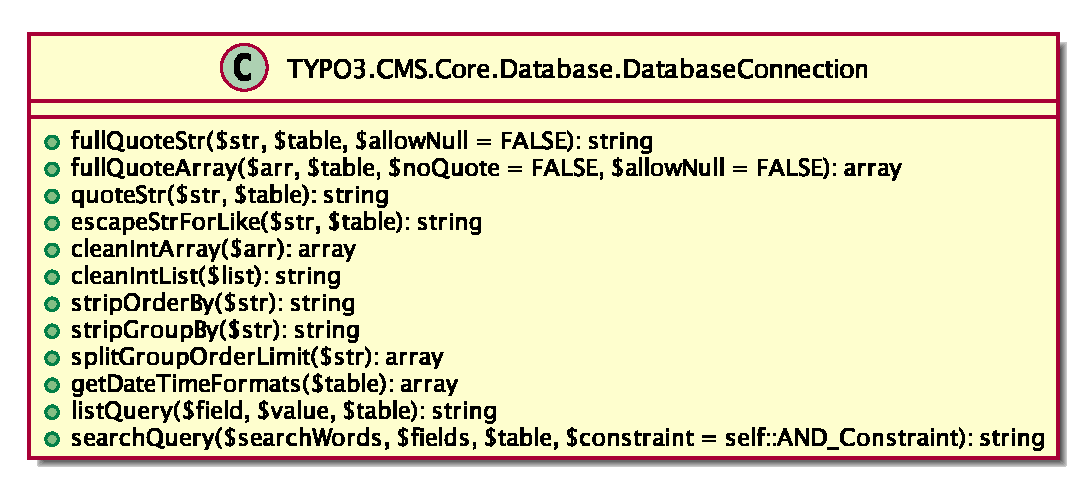
\includegraphics[scale=0.65]{gfx/uml/DatabaseConnectionHelperMethods.eps}
\caption{Hilfsmethoden}
\label{fig:databaseConnectionWithHelperMethods}
\end{figure}

\section{Prepared Statements}
\label{currentsituationsubsec:preparedStatements}
Seit TYPO3 CMS 4.5 können Prepared Statements für \mysqlinline{SELECT} Abfragen verwendet werden. TYPO3 CMS unterstützt sowohl \textit{Posistional Parameters} wie auch \textit{Named Parameters}.

\begin{listing}
\begin{phpcode}
$statement = $GLOBALS['TYPO3_DB']->prepare_SELECTquery(
  '*', 'bugs', 'reported_by = ? AND bug_status = ?'
);
$statement->execute(array('goofy', 'FIXED'));

$statement = $GLOBALS['TYPO3_DB']->prepare_SELECTquery(
  '*', 'bugs', 'reported_by = :nickname AND bug_status = :status'
);
$statement->execute(array(':nickname' => 'goofy', ':status' => 'FIXED'));
\end{phpcode}
\caption{Positional und Named Prepared Statements der TYPO3 CMS Datenbank API}
\label{lst:databaseOldPreparedStatement}
\end{listing}

\phpinline{\TYPO3\CMS\Core\Database\DatabaseConnection::prepare_SELECTquery} liefert ein Objekt der Klasse \phpinline{\TYPO3\CMS\Core\Database\PreparedStatement} zurück, welches sich an der API von \gls{pdo} orientiert.

\begin{figure}[H]
    \centering
    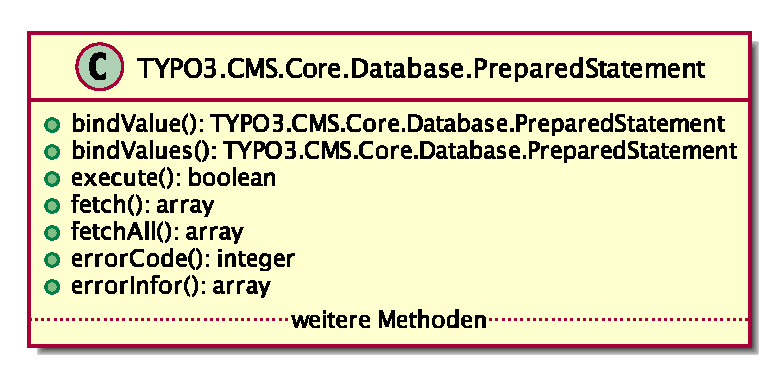
\includegraphics[scale=0.75]{gfx/uml/PreparedStatement.eps}
    \caption{Die Klasse PreparedStatement mit ausgewählten Methoden}
    \label{fig:selectedMethodsOfPreparedStatements}
\end{figure}

\section{Datenbankschema}
\label{currentSituation:subsec:databaseSchema}
Nach der Installation von TYPO3 CMS beinhaltet die Datenbank rund 60 einzelne Tabellen. Die Anzahl hängt von der Installation der optionalen Systemextensions ab.

Wichtige Tabellen sind:
\begin{itemize}
	\item pages – Enthält die Seiten
	\item tt\_content – Enthält die Inhaltselemente, die auf den Seiten dargestellt werden
	\item be\_groups / fe\_groups – Enthält die Backend- beziehungsweise die Nutzergruppen
	\item be\_users / fe\_users – enthält die Backend- beziehungsweise die Frontendbenutzer
\end{itemize}

Dazu kommen Tabellen
\begin{itemize}
	\item die gecachte Daten und Sessions beinhalten,
	\item die der Indexierung des Inhalts dienen
	\item sowie zum Protokollieren von Systemereignissen
\end{itemize}

Die Inhalte werden in TYPO3 CMS in einer Dateisystem ähnlichen Baumstruktur verwaltet. Eine Webseite wird darin durch einen Datensatz vom Typ \textit{Seite} repräsentiert. Dieser Datensatz hat eine ID, die im gleichnamigen Feld in der Tabelle \texttt{pages} gespeichert wird. Diese ist der \textit{Unique Identifier} des Datensatzes.

Die Inhalte einer Webseite wie Texte, Bilder oder Formulare werden innerhalb einer Seite abgelegt. TYPO3 CMS bietet hierzu eine breite Palette von verschiedenen Elementen an. Zudem können Plugins und wiederum Seiten innerhalb eines Seitendatensatzes abgelegt werden. Diese Liste kann unbegrenzt fortgeführt werden, da jede Extension neue Elemente einführen kann, die in einer Seite ablegbar sind. Es ist lediglich wichtig zu wissen, dass Datensätze innerhalb von Seiten abgelegt werden können. Die Inhaltselemente werden hauptsächlich in der Tabelle \texttt{tt\_content} gespeichert beziehungsweise in den Tabellen, die die Extension vorsieht.

\begin{figure}[H]
	\centering
	\includegraphics[scale=0.6]{diagrams/DatabasePagesTTContent.png}
	\caption{Die Tabellen pages und tt\_content}
	\label{fig:pagesAndTTContent}
\end{figure}

Die Verknüpfung von Inhaltselement zu übergeordneter Seite erfolgt in der Datenbank über die Spalte \phpinline{pid} (PageID), in der die ID der übergeordneten Seite als Fremdschlüssel gespeichert wird. Listing~\ref{lst:getSubpages} zeigt die SQL-Abfrage, die alle Unterseiten einer Seite zurückgibt. Dabei hat die Seite, dessen Unterseiten abgefragt werden, die \texttt{uid} 4, die in die Abfrage eingesetzt wird. Die Abfrage lautet: Wähle alle Datensätze aus der Tabelle \texttt{pages}, die in der Spalte \texttt{pid} eine 4 stehen haben.

\begin{listing}
	\begin{phpcode}
SELECT * FROM pages WHERE pid=4 ORDER BY sorting
	\end{phpcode}
	\caption{Abrufen von Unterseiten einer Seite}
	\label{lst:getSubpages}
\end{listing}

Analog zum vorigen Listing, zeigt das Folgende die SQL-Abfrage, die alle Inhaltselemente von der Datenbank abfragt.

\begin{listing}
	\begin{phpcode}
SELECT * FROM tt_content WHERE pid=4 ORDER BY sorting
	\end{phpcode}
	\caption{Abrufen von Inhaltselementen einer Seite}
	\label{lst:getContentElements}
\end{listing}

Die beiden Abfragen geben alle Datensätze zurück, was in der Realität jedoch meistens nicht gewünscht ist. Zum Beispiel sollen keine gelöschten Datensätze angezeigt oder nicht alle Inhaltselemente ausgegeben werden. Datensätze werden in der Datenbank nicht gelöscht, sondern in der Spalte \textit{deleted} durch das setzen des Wertes auf 1 als gelöscht markiert. Inhaltselemente werden über die Spalte \texttt{CType} nach ihrem Typ gefiltert. Um das gewünschte Ergebnis zu erhalten müssen \mysqlinline{WHERE}-Klauseln formuliert werden, was die doch recht trivialen SQL-Abfragen schnell komplex werden lässt.

In TYPO3 CMS können die Benutzerrechte sehr granular eingestellt werden. Die Einstellungen können per Benutzer oder Benutzergruppe vorgenommen werden.
Dabei kann ein Benutzer Mitglied keiner, einer oder mehrerer Benutzergruppen sein. Zudem kann eine Benutzergruppe keinen, einen oder mehrere Benutzer enthalten. Dies stellt eine Many-to-Many-Relation dar.

In der Datenbank wird die Zugehörigkeit von Benutzer zu Gruppe von den Tabellen \texttt{fe\_users} und \texttt{fe\_groups} beziehungsweise \texttt{be\_users} und \texttt{be\_groups} abgebildet.

\begin{figure}[H]
	\centering
	\includegraphics[scale=0.6]{diagrams/DatabaseBEUserGroup.png}
	\caption{Die Tabellen be\_users und be\_groups}
	\label{fig:beUsersAndBeGroups}
\end{figure}

In Abbildung~\ref{fig:beUsersAndBeGroups} fällt der Datentyp der Spalte \texttt{usergroup} auf, der die ID der Gruppe des Benutzers speichert. Er wurde als Typ \mysqlinline{VARCHAR} definiert, obwohl die Spalte \texttt{uid} den Typ \mysqlinline{INT} hat. Dies liegt darin, dass die Zuordnung der Benutzer zu Gruppe über eine kommaseparierte Liste erfolgt:

\begin{table}[H]
\begin{Verbatim}[samepage=true]
+----+-----+------------+----------+----------+-------+-----------+---------+
| id | pid |   tstamp   | username | password | admin | usergroup | deleted |
+----+-----+------------+----------+----------+-------+-----------+---------+
|  1 |  0  | 1191353353 | admin    |  secret  |   1   |           |    0    |
|  2 |  0  | 1281556682 | snape    |  secret  |   1   |    43     |    0    |
|  3 |  0  | 1191353353 | hagrid   |  secret  |   0   |  5,32,43  |    0    |
+----+-----+------------+----------+----------+-------+-----------+---------+
\end{Verbatim}
\caption{Auszug aus der be\_users Tabelle}
\label{tab:tableBeUser}
\end{table}

Kommaseparierte Listen gibt es an vielen Stellen in der Datenbank. Die API von TYPO3 CMS stellt Methoden bereit, die die Liste für die weitere Verarbeitung aufbereiten.

Dieses Konstrukt existiert wahrscheinlich seit Beginn des Systems und es ist zu vermuten, dass damit eine Many-to-Many-Tabelle vermieden werden sollte, was die Komplexität der SQL-Abfrage erhöht.

Um die kommaseparierten Listen aufzulösen, müsste eine weitere Tabelle eingeführt werden, deren zwei Spalten jeweils auf die \texttt{id} der beiden zu verknüpfenden Tabellen referenzieren.

\begin{figure}[H]
	\centering
	\includegraphics[scale=0.6]{diagrams/DatabaseBEUserGroupMM.png}
	\caption{Normalisierung über Many-to-Many Tabelle}
	\label{fig:beUsersHasBeGroups}
\end{figure}

\begin{table}[H]
\begin{Verbatim}[samepage=true]
+--------------+---------------+
| be_users_uid | be_groups_uid |
+--------------+---------------+
|      2       |      34       |
|      3       |       5       |
|      3       |      32       |
|      3       |      43       |
+--------------+---------------+
\end{Verbatim}
\caption{Die MM-Tabelle für be\_users}
\label{tab:mmTableBeUser}
\end{table}

TYPO3 CMS nutzt weder Datenbankseitige \textit{Constraints} noch Fremdschlüssel Definitionen. Alle Referenzierungen werden von TYPO3 CMS selbst verwaltet.

		%-----------------------------------------------
% Dateiname: Protype.tex
% Autor    : Stefano Kowalke <blueduck@gmx.net>
% Lizenz   : BSD
%-----------------------------------------------
\chapter{Prototypischer Nachweis der Herstellbarkeit}
\label{ch:protoype}

\section{Refactoring der alten Datenbank API}
\subsection{Tests für die alte Datenbank API}

\section{Testgetriebene Implementierung der neuen Datenbank API}
- Adapter
- alte API Klasse erbt von neuer API Klasse
- Verbindung mit der Datenbank via Doctrine
- Methodenübername wenn sinnvoll
- Neue Methoden

\subsection{Einführung von Query Objekten}
\subsubsection{SELECT}
\subsubsection{INSERT}
\subsubsection{UPDATE}
\subsubsection{DELETE}
\subsubsection{TRUNCATE}

\section{Anwendung der neuen Datenbank API}
%\subsection{Anpassungen an TYPO3}
\section{Überprüfen der Funktionalität}

		%%-----------------------------------------------
% Dateiname: Outlook.tex
% Autor    : Stefano Kowalke <blueduck@gmx.net>
% Lizenz   : BSD
%-----------------------------------------------
\chapter{Ausblick}
\label{ch:outlook}
\begin{itemize}
	\item{Einladung zum ACME14N}
	\item{Einbau in den Core}
	\item{Nutzung von Doctrine Migrations}
	\item{Nutzung von Doctrine ORM}
	\item{Umbau der Datenbankobjekts zu einem Datenbankconnection Pool}
	Design Pattern Static Fabric oder Fabric
\end{itemize}

	\backmatter
		%-----------------------------------------------
% Dateiname: Conclusion.tex
% Autor    : Stefano Kowalke <blueduck@gmx.net>
% Lizenz   : BSD
%-----------------------------------------------
\chapter{Zusammenfassung}
\label{ch:conclusion}

	\appendix
		\printbibliography[title={Quellenverzeichnis}]
		\includepdfset{pagecommand={\thispagestyle{headings}}}
		% Print glossar
		\printglossary[type=main,title=Glossar,toctitle=Glossar,style=altlist]
		% Print Akronyms
		\printglossary[type=\acronymtype, title=Abkürzungsverzeichnis,toctitle=Abk\"urzungsverzeichnis,style=long]% Der Umlaut muß hier so angegeben werden, da es sonst Anzeigeprobleme im PDF-Viewer gibt.
		\listoftables
		\listoffigures
		\listoflistings
		\includepdf[pages={1,2}, addtotoc={1,chapter,0,Tabelle alte API Methoden - neue Methoden,chap:int},  scale=0.9]{Bib/Functions.pdf}
		%-----------------------------------------------
% Dateiname: Statement.tex
% Autor    : Stefano Kowalke <blueduck@gmx.net>
% Lizenz   : BSD
%-----------------------------------------------
\chapter{Eidesstattliche Erkl\"arung}
\label{ch:erklaerung}

Ich versichere, dass ich die vorliegende Thesis ohne fremde Hilfe selbstständig verfasst und nur die angegebenen Quellen benutzt habe.
\vspace*{2em}
\\
\myLocation, den \today \\\\

\underline{\ \ \ \ \ \ \ \ \ \ \ \ \ \ \ \ \ \ \ \ \ \ \ \ \ \ \ \ }\\\\
\small{\myName}

		% Glossaries und Akronyme kommen hier hin oder ins Frontmatter
\end{document}
